%Chapter 3
\chapter{Developing a simulation methodology}
\thispagestyle{empty}
\vspace{40em}
\hrulefill
\\
\enquote{\textit{Great Design is iteration of good design.}} - Dr M. Cobanli\\
\newpage
\section{Introduction}
This chapter provides details about the development and implementation methodology of simulations to optimise compressed air systems in the mining industry. The method that was developed uses insights gathered from the literature that had bee reviewed (see \Cref{Chap2}). The \gls{ptb} simulation software was used for this study. However, the methodology can be adapted for an equivalent alternative tool.
\par 
Implementation of a simulation model is divided into three steps as shown in the flow diagram in \Cref{fig: Methodology}. Firstly, the specific air network is investigated. The data acquired from the system survey is then utilised to develop and verify a simulation model. In the final step, scenarios are tested using simulations. The results are then quantified and prioritised. After the process has been reviewed, a simulation report is then produced and given to the responsible mine personnel. Each step will be discussed in more detail in the section that follows.

\begin{figure}[h]
	\centering
	\fbox{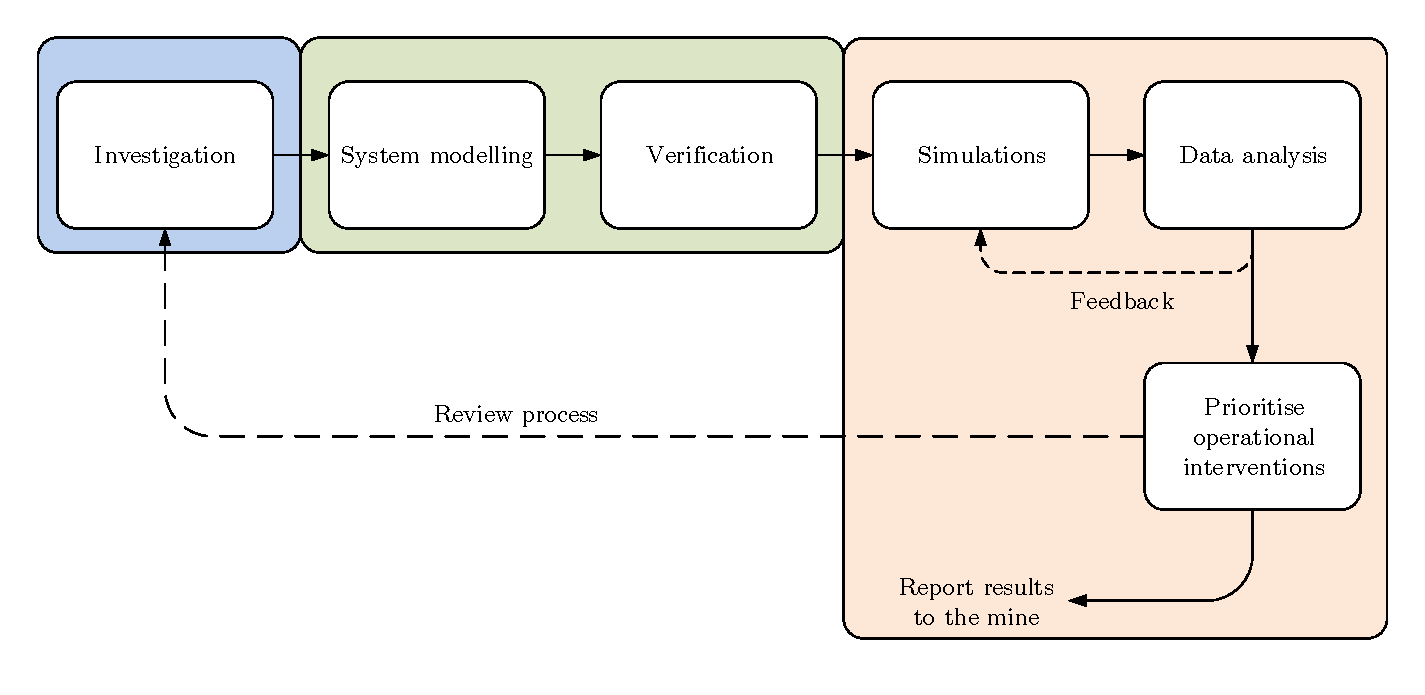
\includegraphics[trim=0.5cm 0.8cm 0.5cm 0.5cm,width=0.98\textwidth]{Graphs/3/Methodology/Methodology.pdf}}
	\caption{Flow diagram of the methodology for this study}
	\label{fig: Methodology}
\end{figure}
\section{Investigate the system}
	\subsection{Preamble}
		Developing a detailed simulation model of a compressed air network requires thorough comprehension of the inner workings of the system. This section will discuss the investigations needed to obtain the required understanding.
	\subsection{Acquire data} % 
	The first step in investigating the system is to acquire the data and understanding that will be required to model the functioning of a compressed air system. Such a system survey will need access to resources such as data storage systems, instrumentation, and communication with relevant engineers and personnel.
	\par 
	Comprehensive and up-to-date process layouts illustrate a compressed air network's unique set-up, scale and the location of instrumentation. More detailed layouts can provide per-level air consumption breakdowns of the network, refuge bays areas, mining cross-sections and identified inefficiencies. The layouts are vital to understand the system process and identify what data parameters will be required for the simulation model. 
	\par 
	A baseline period\footnote{A period that best reflects the typical operation before implementation of an energy intervention. This period is then compared with a period post-intervention implementation to determine the improvements.} that best represents the typical operation of the mine must be selected. Furthermore, availability of data should be considered. The length of the baseline period is selected based on the scenarios that are to be tested; this can be changed later. For calibrating a compressed air system, a 24-hour period of normal operation is usually sufficient. A longer period may be needed to verify the model. 

	\subsection{Investigate mining schedules}
	A critical aspect of developing an accurate model of a mining compressed air system is to take note of the operational philosophy of the mine. The schedule for operations such as drilling, blasting or cleaning may have a major impact on compressed air requirements at different times of the day. By utilising the operational schedule, simulation scenarios can be optimised for the different air requirements throughout the day.	
	
	\subsection{Verify data accuracy}
	Data verification involves a process where data is evaluated to ensure accuracy. It is important to verify data that is used for model development as an accurate representation of the operation of a system can only be achieved if data of high quality is used \cite{gous2016data}. The factors that influence a dataset's quality, accuracy and integrity can be summarised as follows:
	\begin{itemize}
		\item Conversion of measurement value \cite{meijsen2015verification}
		\item Storage and collection of the system \cite{vanNiekerk2016quantification}, \cite{Jansevan2016structuring}
		\item Traceability of measurement sources \cite{Jansevan2016structuring}
		\item Measurement equipment accuracy and malfunctions \cite{gous2016data}
		\item Data abnormalities \cite{gous2016data}
	\end{itemize} 
	\par 
	Therefore, a data verification methodology is utilised to ensure that datasets are of a high quality. 
	\subsection{Resolve missing data}
		Data that is required to develop the simulation model, such as flows and pressures, may not be actively logged by mine systems. It is often necessary to investigate alternative sources and methods to obtain the data. For example, for process elements where instrumentation is absent, estimations can be made based on assumptions regarding instrumentation on the network or based on spot inspections.
		\par 
		Air network specifications such as piping sizes, technical layouts, major leak locations or specifications are often outdated or not recorded. Critical data should be obtained through audits and inspections of the system. If a manual inspection is not possible, estimations should be made from the available data. %\texttt{REMEMBER TO REFERENCE\\ SPECIFIC LOCATION LITERATURE}.
	
	\subsection{Summary}	
	This section discussed the method to investigate a compressed air system. It described the processes for acquiring data and information regarding the specific compressed air network, the process to evaluate and authenticate data accuracy, as well as the procedures for dealing with situations where no data is available.
\section{Develop and verify a simulation model}
	\subsection{Preamble}
	Compressed air networks are comprised of components such as compressors, valves, pipes and other components. This section will discuss the development, calibration and verification of component models that make up a compressed air simulation model. 
	
	\subsection{Select the process boundaries and simulation parameters}
	The simulation boundaries determine the detail based on which the system process is modelled. For a simple compressed air model, the boundaries can be set around the compressor house. This model would then include only the compressor components, inlet and outlet air flows. Alternatively, a more complex model can be developed by choosing boundaries to include more aspects of the process such as specific flows on mining levels.\par 
	 \begin{figure}[h]
	 	\centering
	 	\fbox{\hspace{0.05\textwidth}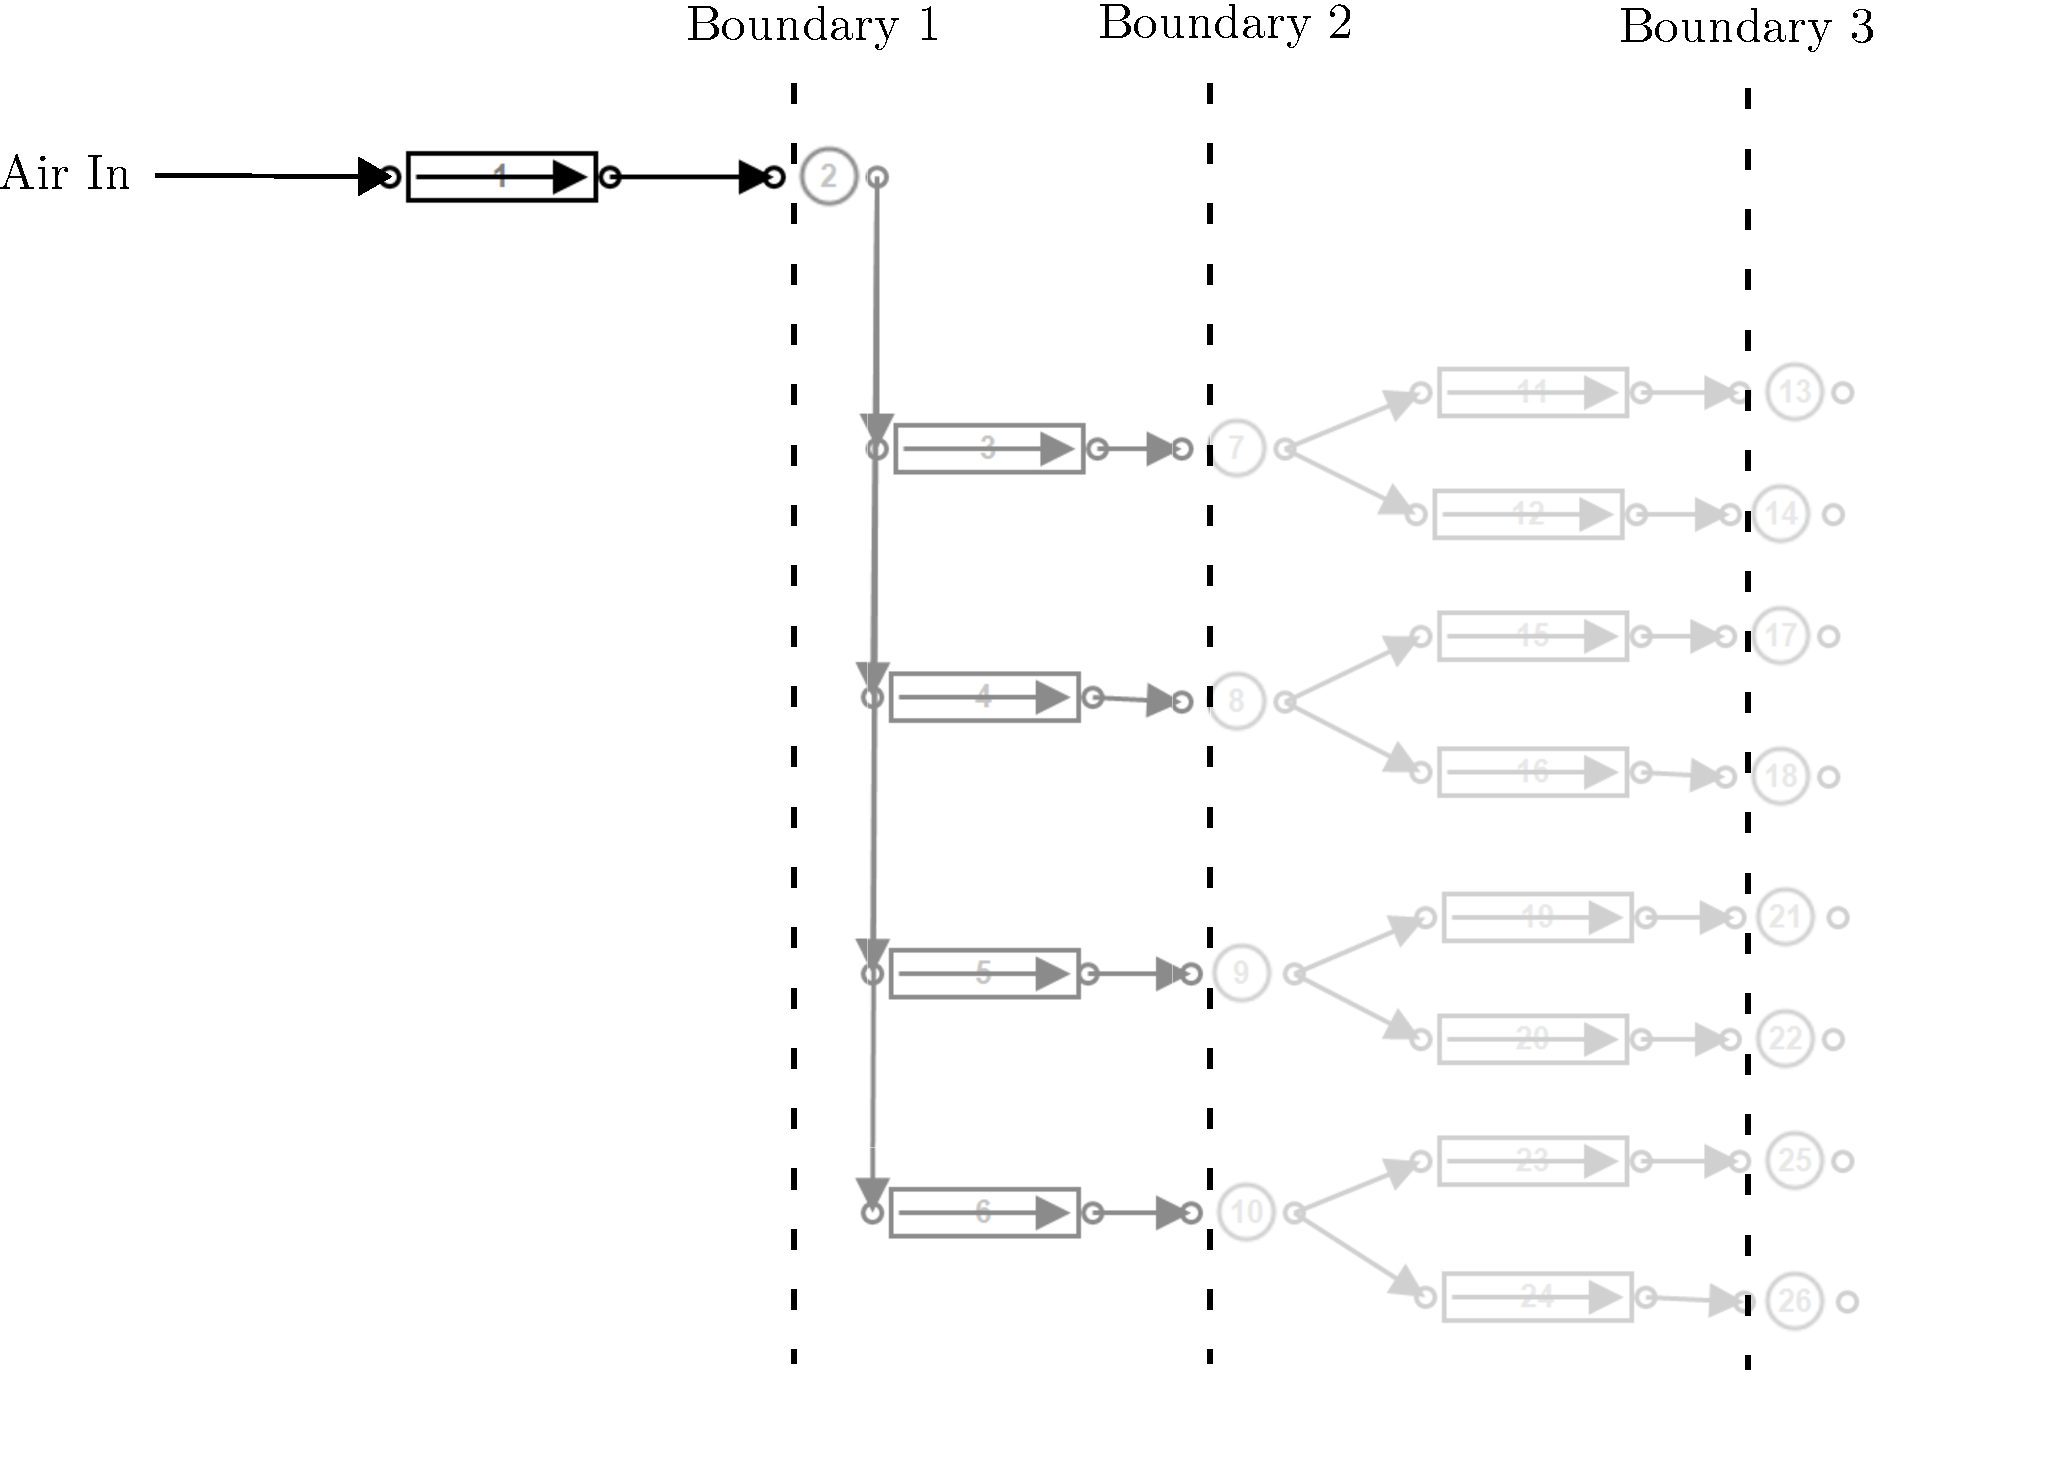
\includegraphics[width=0.88\textwidth]{Images/3/Detail.pdf}\hspace{0.05\textwidth}}
	 	\caption{Selecting boundaries for the simulation model}
	 	\label{fig: Sensitivity}
	 \end{figure}
	The process boundaries should be selected based on the input data available, the accuracy targets and the available time and resources. A more detailed model will allow more accurate simulation. However, it may take more time and resources to obtain the data required to calibrate the model. \Cref{fig: Sensitivity} shows an example of different boundary selection for the same system.
	\par
	Period and data step sizes of the simulation is just as important. The period or duration of the simulation should be determined to ensure that the effects of a scenario are fully tested. Most commonly, previous studies have simulated a "typical" 24 hour period of operation. Most mining compressed air systems follow daily trends and patterns. Therefore, there is no need to simulate a longer period as day to day results would be very similar. A longer simulation may be required for cases where the system operation varies from day to day.
	\par 
	The simulation step size indicates the data resolution. A lower step size will result in a more accurate simulation of the system. However, the processing and data analysis is effected. In this study, the smallest available step size\footnote{The minimum step size is determined from the logging interval of the input data instrumentation. For example, if all input data is logged at 10-minute intervals, the minimum step size would be 10 minutes.} is selected to ensure that the simulated results achieve the desired precision. 
	\par 
	 Compressed air processes such as opening/closing valves or compressors stopping or starting may occur within minutes or seconds. Therefore, higher step sizes (30+ min.) sizes may delay process changes. This delay makes replication of the system control more difficult which reduces simulation accuracy.
	\par
	A higher time-step resolution allows for more precise tuning of controllers and dynamic components. If input data is not available at the desired resolution, the data can be interpolated using the appropriate method. An example of the application of linear interpolation to increase the time-step resolution as shown in \Cref{fig: Inter}. However, incorrectly estimating the \enquote{in-between}  data value may adversely affect the simulation accuracy.
	
	\begin{figure}[h]
		\centering
		\fbox{% GNUPLOT: LaTeX picture with Postscript
\begingroup
  \makeatletter
  \providecommand\color[2][]{%
    \GenericError{(gnuplot) \space\space\space\@spaces}{%
      Package color not loaded in conjunction with
      terminal option `colourtext'%
    }{See the gnuplot documentation for explanation.%
    }{Either use 'blacktext' in gnuplot or load the package
      color.sty in LaTeX.}%
    \renewcommand\color[2][]{}%
  }%
  \providecommand\includegraphics[2][]{%
    \GenericError{(gnuplot) \space\space\space\@spaces}{%
      Package graphicx or graphics not loaded%
    }{See the gnuplot documentation for explanation.%
    }{The gnuplot epslatex terminal needs graphicx.sty or graphics.sty.}%
    \renewcommand\includegraphics[2][]{}%
  }%
  \providecommand\rotatebox[2]{#2}%
  \@ifundefined{ifGPcolor}{%
    \newif\ifGPcolor
    \GPcolortrue
  }{}%
  \@ifundefined{ifGPblacktext}{%
    \newif\ifGPblacktext
    \GPblacktextfalse
  }{}%
  % define a \g@addto@macro without @ in the name:
  \let\gplgaddtomacro\g@addto@macro
  % define empty templates for all commands taking text:
  \gdef\gplbacktext{}%
  \gdef\gplfronttext{}%
  \makeatother
  \ifGPblacktext
    % no textcolor at all
    \def\colorrgb#1{}%
    \def\colorgray#1{}%
  \else
    % gray or color?
    \ifGPcolor
      \def\colorrgb#1{\color[rgb]{#1}}%
      \def\colorgray#1{\color[gray]{#1}}%
      \expandafter\def\csname LTw\endcsname{\color{white}}%
      \expandafter\def\csname LTb\endcsname{\color{black}}%
      \expandafter\def\csname LTa\endcsname{\color{black}}%
      \expandafter\def\csname LT0\endcsname{\color[rgb]{1,0,0}}%
      \expandafter\def\csname LT1\endcsname{\color[rgb]{0,1,0}}%
      \expandafter\def\csname LT2\endcsname{\color[rgb]{0,0,1}}%
      \expandafter\def\csname LT3\endcsname{\color[rgb]{1,0,1}}%
      \expandafter\def\csname LT4\endcsname{\color[rgb]{0,1,1}}%
      \expandafter\def\csname LT5\endcsname{\color[rgb]{1,1,0}}%
      \expandafter\def\csname LT6\endcsname{\color[rgb]{0,0,0}}%
      \expandafter\def\csname LT7\endcsname{\color[rgb]{1,0.3,0}}%
      \expandafter\def\csname LT8\endcsname{\color[rgb]{0.5,0.5,0.5}}%
    \else
      % gray
      \def\colorrgb#1{\color{black}}%
      \def\colorgray#1{\color[gray]{#1}}%
      \expandafter\def\csname LTw\endcsname{\color{white}}%
      \expandafter\def\csname LTb\endcsname{\color{black}}%
      \expandafter\def\csname LTa\endcsname{\color{black}}%
      \expandafter\def\csname LT0\endcsname{\color{black}}%
      \expandafter\def\csname LT1\endcsname{\color{black}}%
      \expandafter\def\csname LT2\endcsname{\color{black}}%
      \expandafter\def\csname LT3\endcsname{\color{black}}%
      \expandafter\def\csname LT4\endcsname{\color{black}}%
      \expandafter\def\csname LT5\endcsname{\color{black}}%
      \expandafter\def\csname LT6\endcsname{\color{black}}%
      \expandafter\def\csname LT7\endcsname{\color{black}}%
      \expandafter\def\csname LT8\endcsname{\color{black}}%
    \fi
  \fi
    \setlength{\unitlength}{0.0500bp}%
    \ifx\gptboxheight\undefined%
      \newlength{\gptboxheight}%
      \newlength{\gptboxwidth}%
      \newsavebox{\gptboxtext}%
    \fi%
    \setlength{\fboxrule}{0.5pt}%
    \setlength{\fboxsep}{1pt}%
\begin{picture}(9200.00,4032.00)%
    \gplgaddtomacro\gplbacktext{%
      \colorrgb{0.00,0.00,0.00}%
      \put(682,924){\makebox(0,0)[r]{\strut{}$0$}}%
      \colorrgb{0.00,0.00,0.00}%
      \put(682,1303){\makebox(0,0)[r]{\strut{}$2$}}%
      \colorrgb{0.00,0.00,0.00}%
      \put(682,1682){\makebox(0,0)[r]{\strut{}$4$}}%
      \colorrgb{0.00,0.00,0.00}%
      \put(682,2061){\makebox(0,0)[r]{\strut{}$6$}}%
      \colorrgb{0.00,0.00,0.00}%
      \put(682,2440){\makebox(0,0)[r]{\strut{}$8$}}%
      \colorrgb{0.00,0.00,0.00}%
      \put(682,2819){\makebox(0,0)[r]{\strut{}$10$}}%
      \colorrgb{0.00,0.00,0.00}%
      \put(682,3198){\makebox(0,0)[r]{\strut{}$12$}}%
      \colorrgb{0.00,0.00,0.00}%
      \put(682,3577){\makebox(0,0)[r]{\strut{}$14$}}%
      \colorrgb{0.00,0.00,0.00}%
      \put(814,704){\makebox(0,0){\strut{}00:00}}%
      \colorrgb{0.00,0.00,0.00}%
      \put(2172,704){\makebox(0,0){\strut{}04:00}}%
      \colorrgb{0.00,0.00,0.00}%
      \put(3530,704){\makebox(0,0){\strut{}08:00}}%
      \colorrgb{0.00,0.00,0.00}%
      \put(4888,704){\makebox(0,0){\strut{}12:00}}%
      \colorrgb{0.00,0.00,0.00}%
      \put(6246,704){\makebox(0,0){\strut{}16:00}}%
      \colorrgb{0.00,0.00,0.00}%
      \put(7604,704){\makebox(0,0){\strut{}20:00}}%
      \colorrgb{0.00,0.00,0.00}%
      \put(8962,704){\makebox(0,0){\strut{}00:00}}%
    }%
    \gplgaddtomacro\gplfronttext{%
      \csname LTb\endcsname%
      \put(176,2345){\rotatebox{-270}{\makebox(0,0){\strut{}c/kWh}}}%
      \put(4888,374){\makebox(0,0){\strut{}Time of Day}}%
      \csname LTb\endcsname%
      \put(4133,173){\makebox(0,0)[r]{\strut{}Interpolated datset}}%
      \csname LTb\endcsname%
      \put(7496,173){\makebox(0,0)[r]{\strut{}Orginal dataset}}%
    }%
    \gplbacktext
    \put(0,0){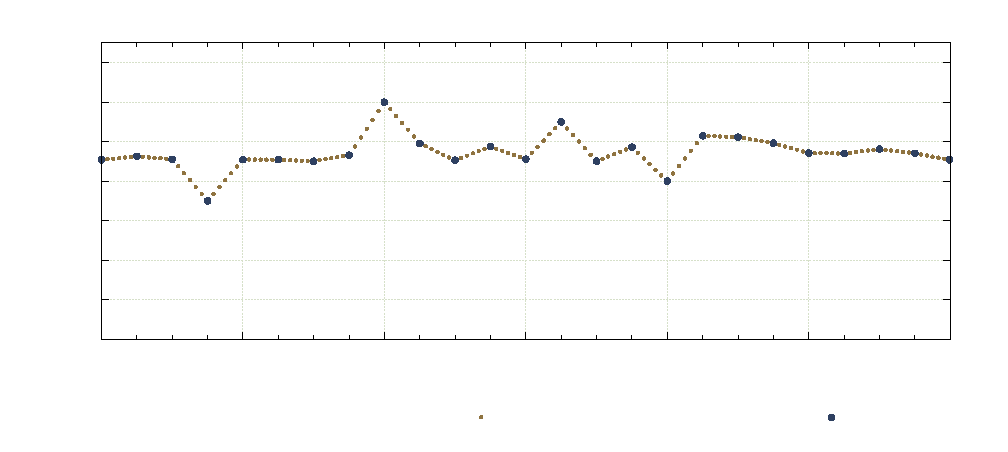
\includegraphics{Graphs/3/inter/inter}}%
    \gplfronttext
  \end{picture}%
\endgroup
}
		\caption{Interpolating input data to increase time-step resolution}
		\label{fig: Inter}
	\end{figure}
	\subsection{Model compressed air network components}
		\subsubsection{Ambient conditions}
		Ambient air condition underground and on the surface change the characteristics of the air, affecting the operation of the system. \Cref{fig: Ambient} shows the average summer air conditions. If no data is available for the specific simulation period, the conditions can be estimated by scaling this profile.
		\begin{figure}[h!]
			\centering
			\fbox{% GNUPLOT: LaTeX picture with Postscript
\begingroup
  \makeatletter
  \providecommand\color[2][]{%
    \GenericError{(gnuplot) \space\space\space\@spaces}{%
      Package color not loaded in conjunction with
      terminal option `colourtext'%
    }{See the gnuplot documentation for explanation.%
    }{Either use 'blacktext' in gnuplot or load the package
      color.sty in LaTeX.}%
    \renewcommand\color[2][]{}%
  }%
  \providecommand\includegraphics[2][]{%
    \GenericError{(gnuplot) \space\space\space\@spaces}{%
      Package graphicx or graphics not loaded%
    }{See the gnuplot documentation for explanation.%
    }{The gnuplot epslatex terminal needs graphicx.sty or graphics.sty.}%
    \renewcommand\includegraphics[2][]{}%
  }%
  \providecommand\rotatebox[2]{#2}%
  \@ifundefined{ifGPcolor}{%
    \newif\ifGPcolor
    \GPcolortrue
  }{}%
  \@ifundefined{ifGPblacktext}{%
    \newif\ifGPblacktext
    \GPblacktextfalse
  }{}%
  % define a \g@addto@macro without @ in the name:
  \let\gplgaddtomacro\g@addto@macro
  % define empty templates for all commands taking text:
  \gdef\gplbacktext{}%
  \gdef\gplfronttext{}%
  \makeatother
  \ifGPblacktext
    % no textcolor at all
    \def\colorrgb#1{}%
    \def\colorgray#1{}%
  \else
    % gray or color?
    \ifGPcolor
      \def\colorrgb#1{\color[rgb]{#1}}%
      \def\colorgray#1{\color[gray]{#1}}%
      \expandafter\def\csname LTw\endcsname{\color{white}}%
      \expandafter\def\csname LTb\endcsname{\color{black}}%
      \expandafter\def\csname LTa\endcsname{\color{black}}%
      \expandafter\def\csname LT0\endcsname{\color[rgb]{1,0,0}}%
      \expandafter\def\csname LT1\endcsname{\color[rgb]{0,1,0}}%
      \expandafter\def\csname LT2\endcsname{\color[rgb]{0,0,1}}%
      \expandafter\def\csname LT3\endcsname{\color[rgb]{1,0,1}}%
      \expandafter\def\csname LT4\endcsname{\color[rgb]{0,1,1}}%
      \expandafter\def\csname LT5\endcsname{\color[rgb]{1,1,0}}%
      \expandafter\def\csname LT6\endcsname{\color[rgb]{0,0,0}}%
      \expandafter\def\csname LT7\endcsname{\color[rgb]{1,0.3,0}}%
      \expandafter\def\csname LT8\endcsname{\color[rgb]{0.5,0.5,0.5}}%
    \else
      % gray
      \def\colorrgb#1{\color{black}}%
      \def\colorgray#1{\color[gray]{#1}}%
      \expandafter\def\csname LTw\endcsname{\color{white}}%
      \expandafter\def\csname LTb\endcsname{\color{black}}%
      \expandafter\def\csname LTa\endcsname{\color{black}}%
      \expandafter\def\csname LT0\endcsname{\color{black}}%
      \expandafter\def\csname LT1\endcsname{\color{black}}%
      \expandafter\def\csname LT2\endcsname{\color{black}}%
      \expandafter\def\csname LT3\endcsname{\color{black}}%
      \expandafter\def\csname LT4\endcsname{\color{black}}%
      \expandafter\def\csname LT5\endcsname{\color{black}}%
      \expandafter\def\csname LT6\endcsname{\color{black}}%
      \expandafter\def\csname LT7\endcsname{\color{black}}%
      \expandafter\def\csname LT8\endcsname{\color{black}}%
    \fi
  \fi
    \setlength{\unitlength}{0.0500bp}%
    \ifx\gptboxheight\undefined%
      \newlength{\gptboxheight}%
      \newlength{\gptboxwidth}%
      \newsavebox{\gptboxtext}%
    \fi%
    \setlength{\fboxrule}{0.5pt}%
    \setlength{\fboxsep}{1pt}%
\begin{picture}(9360.00,4032.00)%
    \gplgaddtomacro\gplbacktext{%
      \colorrgb{0.00,0.00,0.00}%
      \put(682,924){\makebox(0,0)[r]{\strut{}$10$}}%
      \colorrgb{0.00,0.00,0.00}%
      \put(682,1493){\makebox(0,0)[r]{\strut{}$15$}}%
      \colorrgb{0.00,0.00,0.00}%
      \put(682,2061){\makebox(0,0)[r]{\strut{}$20$}}%
      \colorrgb{0.00,0.00,0.00}%
      \put(682,2630){\makebox(0,0)[r]{\strut{}$25$}}%
      \colorrgb{0.00,0.00,0.00}%
      \put(682,3198){\makebox(0,0)[r]{\strut{}$30$}}%
      \colorrgb{0.00,0.00,0.00}%
      \put(682,3767){\makebox(0,0)[r]{\strut{}$35$}}%
      \colorrgb{0.00,0.00,0.00}%
      \put(814,704){\makebox(0,0){\strut{}00:00}}%
      \colorrgb{0.00,0.00,0.00}%
      \put(2025,704){\makebox(0,0){\strut{}04:00}}%
      \colorrgb{0.00,0.00,0.00}%
      \put(3237,704){\makebox(0,0){\strut{}08:00}}%
      \colorrgb{0.00,0.00,0.00}%
      \put(4448,704){\makebox(0,0){\strut{}12:00}}%
      \colorrgb{0.00,0.00,0.00}%
      \put(5659,704){\makebox(0,0){\strut{}16:00}}%
      \colorrgb{0.00,0.00,0.00}%
      \put(6871,704){\makebox(0,0){\strut{}20:00}}%
      \colorrgb{0.00,0.00,0.00}%
      \put(8082,704){\makebox(0,0){\strut{}00:00}}%
      \colorrgb{0.00,0.00,0.00}%
      \put(8214,924){\makebox(0,0)[l]{\strut{}$0$}}%
      \colorrgb{0.00,0.00,0.00}%
      \put(8214,1493){\makebox(0,0)[l]{\strut{}$20$}}%
      \colorrgb{0.00,0.00,0.00}%
      \put(8214,2061){\makebox(0,0)[l]{\strut{}$40$}}%
      \colorrgb{0.00,0.00,0.00}%
      \put(8214,2630){\makebox(0,0)[l]{\strut{}$60$}}%
      \colorrgb{0.00,0.00,0.00}%
      \put(8214,3198){\makebox(0,0)[l]{\strut{}$80$}}%
      \colorrgb{0.00,0.00,0.00}%
      \put(8214,3767){\makebox(0,0)[l]{\strut{}$100$}}%
    }%
    \gplgaddtomacro\gplfronttext{%
      \csname LTb\endcsname%
      \put(176,2345){\rotatebox{-270}{\makebox(0,0){\strut{}Relative Humidity (\%)}}}%
      \put(8851,2345){\rotatebox{-270}{\makebox(0,0){\strut{}Temperature ()$^\circ C$)}}}%
      \put(4448,374){\makebox(0,0){\strut{}Time of Day}}%
      \csname LTb\endcsname%
      \put(3593,100){\makebox(0,0)[r]{\strut{}Temperature}}%
      \csname LTb\endcsname%
      \put(6692,100){\makebox(0,0)[r]{\strut{}Relative Humidity}}%
    }%
    \gplbacktext
    \put(0,0){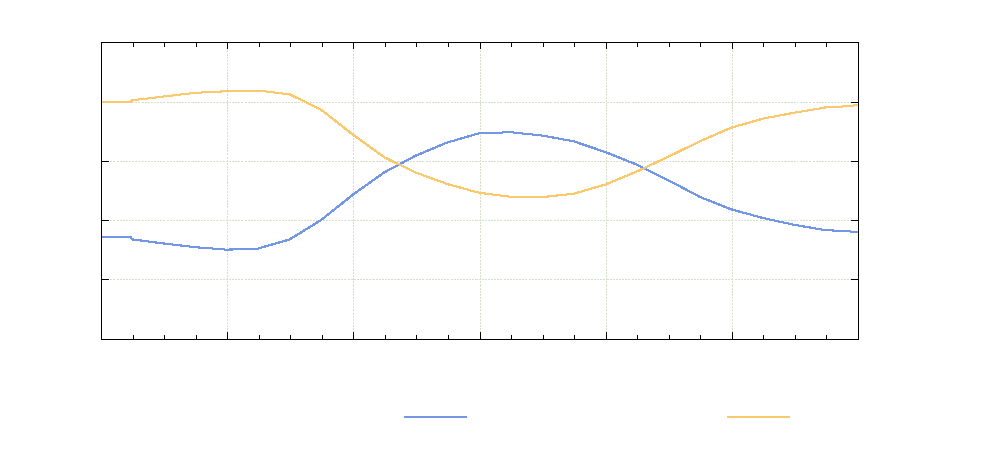
\includegraphics{Graphs/3/Ambient/Ambient}}%
    \gplfronttext
  \end{picture}%
\endgroup
}
			\caption{Average summer ambient air conditions at a South African gold mine}
			\label{fig: Ambient}
		\end{figure}
		\par
		The assumption is made that underground conditions remain constant at each mining level. Pressure and temperature increase with depth as a result of auto compression and rock face temperature. Therefore, the conditions can be estimated using only the depth at each level.
		\subsubsection{Air pipes}
		Pressure losses occur over compressed air networks due to friction within the pipe; these losses should be taken into account in the simulation for large piping networks. A pipe model is used to account for these losses which are defined by the \textit{Darcy-Weisbach equation}\footnote{ B. Glenn, \enquote*{The Darcy–Weisbach Equation,}[Online] \url{https://bae.okstate.edu/faculty-sites/Darcy/DarcyWeisbach/Darcy-WeisbachEq.htm}, [Accessed 20-05-2017]}:
		$$\Delta P = \frac{f L \rho V^2}{2 D}$$
		Where the pressure difference $\Delta P $ is a function of:
		\begin{table}[h!]
			\centering
			\begin{tabular}{cl}
				\hline
				Parameter & Definition\\
				\hline
				$f$ & Friction coefficient \\
				$L$ & Pipe length ($m$) \\
				$D$ & Pipe diameter ($m$) \\
				$\rho$ & Air density ($kg/m^3$)\\	
				$V$ & Average velocity ($m/s$) \\	
				\hline
			\end{tabular} 
			\caption{Air pipe component model parameters}
			\label{table: Darcy-Weisbach}
		\end{table}
		
		The pipe component may be used as a valve by controlling the open fraction between 0 and 1. Modelling the valve flow characteristics is discussed in \Cref{Controllers} \textit{Controllers}.
		
		\subsubsection{Compressors}
		Three compressor models were investigated, each with varying complexity. The models are:
		\begin{itemize}
			\item Air compressor
			\item Dynamic compressor 
			\item Positive displacement compressor
		\end{itemize} 
		The air compressor is a general, simplified model. It requires minimal user inputs by making several assumptions. This model is useful when parameters for a compressor are not available. Alternatively, the air compressor model is ideal when doing a quick or preliminary simulation. However, it is not ideal for detailed simulations which require more precision.
		\par 
		The dynamic compressor components are more complex, taking into account factors such as heat generated by the polytropic process and mechanical inefficiencies. Hence, the model can be used more accurately and for more complex simulations than the general compressor model. However, it should be noted that the dynamic compressor is simplified by several assumptions, for example, a constant efficiency at varying loads. 
		\par 	 
		For most scenarios, the dynamic compressor model is most suitable. This component is modelled by fitting a quadratic curve through three points of operation to obtain an equation for corrected mass flow as a function of the pressure ratio. This characteristic curve of a compressor s shown in \Cref{fig: Compressor Curve} can be accurately estimated even when only one data point is available by making approximations for the zero flow and pressure points on the curve.
		\par
		
		 Once the flow characteristics of the compressors are set, the efficiency and \gls{polyCof} parameters are calibrated such that the output power and air temperature match the actual or estimated outputs of the compressor.
		\par 
		\begin{figure}[h!]
			\centering
			\fbox{% GNUPLOT: LaTeX picture with Postscript
\begingroup
  \makeatletter
  \providecommand\color[2][]{%
    \GenericError{(gnuplot) \space\space\space\@spaces}{%
      Package color not loaded in conjunction with
      terminal option `colourtext'%
    }{See the gnuplot documentation for explanation.%
    }{Either use 'blacktext' in gnuplot or load the package
      color.sty in LaTeX.}%
    \renewcommand\color[2][]{}%
  }%
  \providecommand\includegraphics[2][]{%
    \GenericError{(gnuplot) \space\space\space\@spaces}{%
      Package graphicx or graphics not loaded%
    }{See the gnuplot documentation for explanation.%
    }{The gnuplot epslatex terminal needs graphicx.sty or graphics.sty.}%
    \renewcommand\includegraphics[2][]{}%
  }%
  \providecommand\rotatebox[2]{#2}%
  \@ifundefined{ifGPcolor}{%
    \newif\ifGPcolor
    \GPcolortrue
  }{}%
  \@ifundefined{ifGPblacktext}{%
    \newif\ifGPblacktext
    \GPblacktextfalse
  }{}%
  % define a \g@addto@macro without @ in the name:
  \let\gplgaddtomacro\g@addto@macro
  % define empty templates for all commands taking text:
  \gdef\gplbacktext{}%
  \gdef\gplfronttext{}%
  \makeatother
  \ifGPblacktext
    % no textcolor at all
    \def\colorrgb#1{}%
    \def\colorgray#1{}%
  \else
    % gray or color?
    \ifGPcolor
      \def\colorrgb#1{\color[rgb]{#1}}%
      \def\colorgray#1{\color[gray]{#1}}%
      \expandafter\def\csname LTw\endcsname{\color{white}}%
      \expandafter\def\csname LTb\endcsname{\color{black}}%
      \expandafter\def\csname LTa\endcsname{\color{black}}%
      \expandafter\def\csname LT0\endcsname{\color[rgb]{1,0,0}}%
      \expandafter\def\csname LT1\endcsname{\color[rgb]{0,1,0}}%
      \expandafter\def\csname LT2\endcsname{\color[rgb]{0,0,1}}%
      \expandafter\def\csname LT3\endcsname{\color[rgb]{1,0,1}}%
      \expandafter\def\csname LT4\endcsname{\color[rgb]{0,1,1}}%
      \expandafter\def\csname LT5\endcsname{\color[rgb]{1,1,0}}%
      \expandafter\def\csname LT6\endcsname{\color[rgb]{0,0,0}}%
      \expandafter\def\csname LT7\endcsname{\color[rgb]{1,0.3,0}}%
      \expandafter\def\csname LT8\endcsname{\color[rgb]{0.5,0.5,0.5}}%
    \else
      % gray
      \def\colorrgb#1{\color{black}}%
      \def\colorgray#1{\color[gray]{#1}}%
      \expandafter\def\csname LTw\endcsname{\color{white}}%
      \expandafter\def\csname LTb\endcsname{\color{black}}%
      \expandafter\def\csname LTa\endcsname{\color{black}}%
      \expandafter\def\csname LT0\endcsname{\color{black}}%
      \expandafter\def\csname LT1\endcsname{\color{black}}%
      \expandafter\def\csname LT2\endcsname{\color{black}}%
      \expandafter\def\csname LT3\endcsname{\color{black}}%
      \expandafter\def\csname LT4\endcsname{\color{black}}%
      \expandafter\def\csname LT5\endcsname{\color{black}}%
      \expandafter\def\csname LT6\endcsname{\color{black}}%
      \expandafter\def\csname LT7\endcsname{\color{black}}%
      \expandafter\def\csname LT8\endcsname{\color{black}}%
    \fi
  \fi
    \setlength{\unitlength}{0.0500bp}%
    \ifx\gptboxheight\undefined%
      \newlength{\gptboxheight}%
      \newlength{\gptboxwidth}%
      \newsavebox{\gptboxtext}%
    \fi%
    \setlength{\fboxrule}{0.5pt}%
    \setlength{\fboxsep}{1pt}%
\begin{picture}(9360.00,4032.00)%
    \gplgaddtomacro\gplbacktext{%
      \colorrgb{0.00,0.00,0.00}%
      \put(814,704){\makebox(0,0)[r]{\strut{}$0$}}%
      \colorrgb{0.00,0.00,0.00}%
      \put(814,1261){\makebox(0,0)[r]{\strut{}$100$}}%
      \colorrgb{0.00,0.00,0.00}%
      \put(814,1818){\makebox(0,0)[r]{\strut{}$200$}}%
      \colorrgb{0.00,0.00,0.00}%
      \put(814,2375){\makebox(0,0)[r]{\strut{}$300$}}%
      \colorrgb{0.00,0.00,0.00}%
      \put(814,2932){\makebox(0,0)[r]{\strut{}$400$}}%
      \colorrgb{0.00,0.00,0.00}%
      \put(814,3489){\makebox(0,0)[r]{\strut{}$500$}}%
      \colorrgb{0.00,0.00,0.00}%
      \put(946,484){\makebox(0,0){\strut{}$0$}}%
      \colorrgb{0.00,0.00,0.00}%
      \put(1948,484){\makebox(0,0){\strut{}$2$}}%
      \colorrgb{0.00,0.00,0.00}%
      \put(2950,484){\makebox(0,0){\strut{}$4$}}%
      \colorrgb{0.00,0.00,0.00}%
      \put(3952,484){\makebox(0,0){\strut{}$6$}}%
      \colorrgb{0.00,0.00,0.00}%
      \put(4954,484){\makebox(0,0){\strut{}$8$}}%
      \colorrgb{0.00,0.00,0.00}%
      \put(5956,484){\makebox(0,0){\strut{}$10$}}%
      \colorrgb{0.00,0.00,0.00}%
      \put(6958,484){\makebox(0,0){\strut{}$12$}}%
      \colorrgb{0.00,0.00,0.00}%
      \put(7960,484){\makebox(0,0){\strut{}$14$}}%
      \colorrgb{0.00,0.00,0.00}%
      \put(8962,484){\makebox(0,0){\strut{}$16$}}%
      \csname LTb\endcsname%
      \put(5455,3043){\makebox(0,0)[l]{\strut{}$f(x) = -2.586x^2 + 7.788x + 494$}}%
    }%
    \gplgaddtomacro\gplfronttext{%
      \csname LTb\endcsname%
      \put(176,2235){\rotatebox{-270}{\makebox(0,0){\strut{}Mass flow ($kg^3/s/\sqrt(k)/Bar$)}}}%
      \put(4954,154){\makebox(0,0){\strut{}Pressure ratio}}%
    }%
    \gplbacktext
    \put(0,0){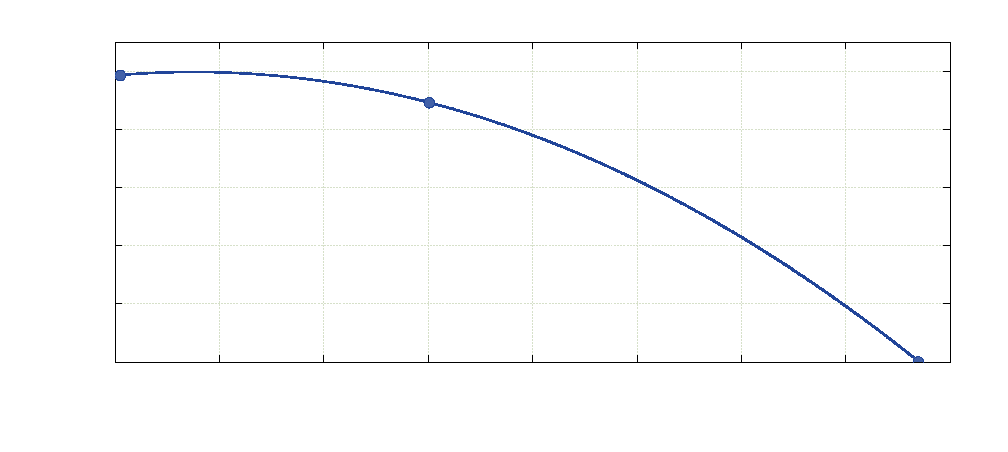
\includegraphics{Graphs/3/AproxCurve/AproxCurve}}%
    \gplfronttext
  \end{picture}%
\endgroup
}
			\caption{Estimating the characteristic curve of a compressor by fitting a quadratic function to points of operation}
			\label{fig: Compressor Curve}
		\end{figure}
		Once the models are accurately calibrated, the compressor component integrates into the air network in the arrangement shown in \Cref{fig: Compressor models}. The Compressor is connected to the inlet air source via an inlet pipe and air node and the rest of the network via an air node and outlet pipe. The additional pipe components allow the inlet and outlet conditions to be monitored and controlled in the simulation.
		\begin{figure}[h]
			\centering
			\fbox{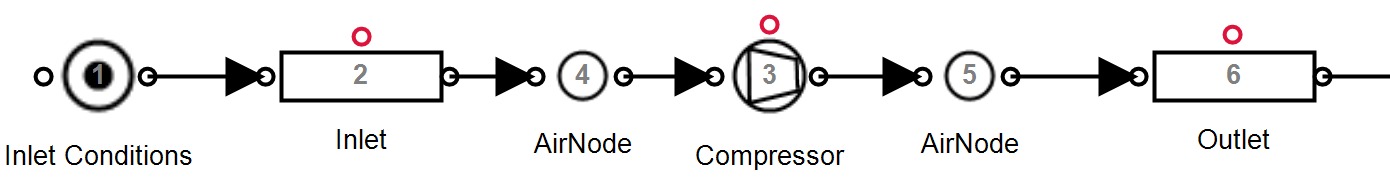
\includegraphics[trim =-4cm 0 -4cm 0cm, width=0.98\textwidth]{Images/3/Compressors}}
			\caption{Integrating the compressor component into the simulation}
			\label{fig: Compressor models}
		\end{figure}		

		\subsubsection{Demand}
			A flow demand represents any air flow leaving the network. Flows leaving the network include any air consuming equipment such as drills and agitators as well as losses like air leaks and open pipes. The air flow is dependent on pressure and the specific resistance to flow of the outlet. 
			\par 
			The resistance of the flow demand can be obtained using the inlet pressure, outlet pressure and flow. If the flow is not known, a reasonably accurate estimation can be made by calculating the expected flow from the size of the outlet. However, his estimation will affect the accuracy.
			\par
			 The air demand may vary throughout the day. For example, a mining section may utilise more machines during certain periods of the day. A schedule and flow profile are used to replicate this in the simulation. \Cref{fig: Demand component} shows how a calibrated air demand or leak is integrated into the simulation model on \gls{ptb}.
			\begin{figure}[h]
				\centering
				\fbox{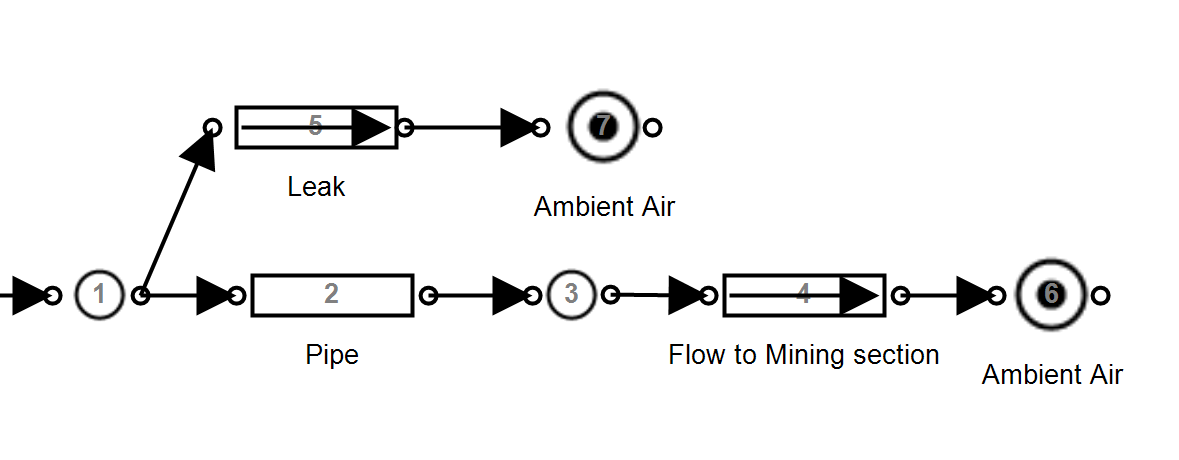
\includegraphics[trim =-12cm 0.5cm -12cm 0.5cm, width=0.98\textwidth]{Images/3/AirDemand}}
				\caption{Implementing flow demands and leaks into the simulation} 
				\label{fig: Demand component}
			\end{figure}
		\subsubsection{Compressed air control}\label{Controllers}
			Simulation components require dynamic control to replicate the operation of the actual air network. Control is typically implemented on compressors and valves throughout the network to follow setpoints and schedules. It is important to not only include the controllers in the simulation but to replicate any nonlinearities, limitations and response delays related to specific types of control. Implementing these control factors will ensure the model reacts in the same way the actual network would, improving accuracy.
			\par 
			On a typical mine, a compressor's power output is controlled to ensure that the discharge pressure matches a specified setpoint. This control is achieved through either \glspl{vsd} (or \glspl{vfd}) and guide vane control. On \gls{ptb} valve or compressor control can be replicated using a \gls{pi} controller as shown in \Cref{fig: Controller models}. For the control system models in \Cref{fig: Controller models}, outlet pressure is used as feedback to the compressor and a valve controller. 
			\par 
			
	\begin{figure}[h!]
		\centering
		\fbox{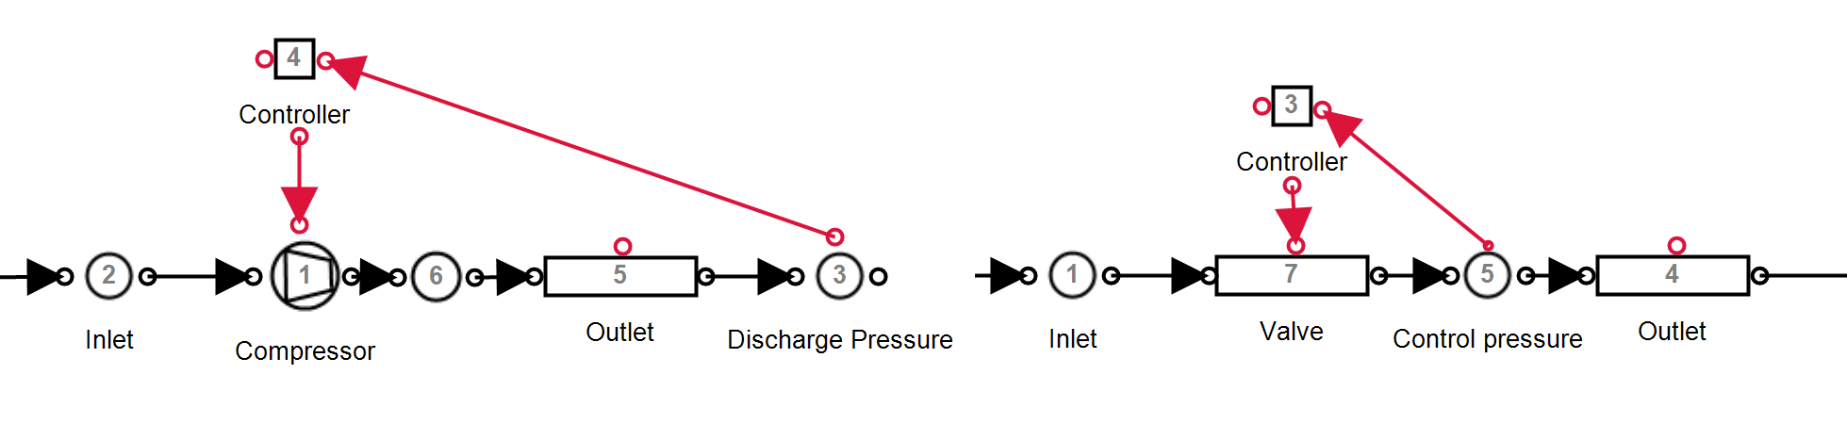
\includegraphics[trim =-4cm 0 -4cm 0cm, width=0.98\textwidth]{Images/3/Controller}}
		\caption[Control components in Process Toolbox]{Control components in Process Toolbox}
		\label{fig: Controller models}
	\end{figure}
		Guide vanes are most commonly used in mining air systems to control compressors. Guide vane control entails controlling the position of the inlet guide vane. The guide vane is opened or closed to control the compressors discharge pressure. Manipulating the guide vane position will affect the output power the compressor inputs into the system. 
		\par 
		\Cref{fig: Guide vane position} shows the relationship between power and guide vane position. A linear relation between guide vane position and compressor output can be used to the estimated effect of guide vane control. The model should take into account the minimum guide vane position limit that is typically set at around 40\% open. As illustrated in \Cref{fig: Guide vane position} this control position maps to an output power for the compressor of about 60\% of the maximum power. When more pressure is required than can be obtained with the guide vanes fully opened, another compressor is needed to operate. 
		\begin{figure}[h]
			\centering
			\fbox{% GNUPLOT: LaTeX picture with Postscript
\begingroup
  \makeatletter
  \providecommand\color[2][]{%
    \GenericError{(gnuplot) \space\space\space\@spaces}{%
      Package color not loaded in conjunction with
      terminal option `colourtext'%
    }{See the gnuplot documentation for explanation.%
    }{Either use 'blacktext' in gnuplot or load the package
      color.sty in LaTeX.}%
    \renewcommand\color[2][]{}%
  }%
  \providecommand\includegraphics[2][]{%
    \GenericError{(gnuplot) \space\space\space\@spaces}{%
      Package graphicx or graphics not loaded%
    }{See the gnuplot documentation for explanation.%
    }{The gnuplot epslatex terminal needs graphicx.sty or graphics.sty.}%
    \renewcommand\includegraphics[2][]{}%
  }%
  \providecommand\rotatebox[2]{#2}%
  \@ifundefined{ifGPcolor}{%
    \newif\ifGPcolor
    \GPcolortrue
  }{}%
  \@ifundefined{ifGPblacktext}{%
    \newif\ifGPblacktext
    \GPblacktextfalse
  }{}%
  % define a \g@addto@macro without @ in the name:
  \let\gplgaddtomacro\g@addto@macro
  % define empty templates for all commands taking text:
  \gdef\gplbacktext{}%
  \gdef\gplfronttext{}%
  \makeatother
  \ifGPblacktext
    % no textcolor at all
    \def\colorrgb#1{}%
    \def\colorgray#1{}%
  \else
    % gray or color?
    \ifGPcolor
      \def\colorrgb#1{\color[rgb]{#1}}%
      \def\colorgray#1{\color[gray]{#1}}%
      \expandafter\def\csname LTw\endcsname{\color{white}}%
      \expandafter\def\csname LTb\endcsname{\color{black}}%
      \expandafter\def\csname LTa\endcsname{\color{black}}%
      \expandafter\def\csname LT0\endcsname{\color[rgb]{1,0,0}}%
      \expandafter\def\csname LT1\endcsname{\color[rgb]{0,1,0}}%
      \expandafter\def\csname LT2\endcsname{\color[rgb]{0,0,1}}%
      \expandafter\def\csname LT3\endcsname{\color[rgb]{1,0,1}}%
      \expandafter\def\csname LT4\endcsname{\color[rgb]{0,1,1}}%
      \expandafter\def\csname LT5\endcsname{\color[rgb]{1,1,0}}%
      \expandafter\def\csname LT6\endcsname{\color[rgb]{0,0,0}}%
      \expandafter\def\csname LT7\endcsname{\color[rgb]{1,0.3,0}}%
      \expandafter\def\csname LT8\endcsname{\color[rgb]{0.5,0.5,0.5}}%
    \else
      % gray
      \def\colorrgb#1{\color{black}}%
      \def\colorgray#1{\color[gray]{#1}}%
      \expandafter\def\csname LTw\endcsname{\color{white}}%
      \expandafter\def\csname LTb\endcsname{\color{black}}%
      \expandafter\def\csname LTa\endcsname{\color{black}}%
      \expandafter\def\csname LT0\endcsname{\color{black}}%
      \expandafter\def\csname LT1\endcsname{\color{black}}%
      \expandafter\def\csname LT2\endcsname{\color{black}}%
      \expandafter\def\csname LT3\endcsname{\color{black}}%
      \expandafter\def\csname LT4\endcsname{\color{black}}%
      \expandafter\def\csname LT5\endcsname{\color{black}}%
      \expandafter\def\csname LT6\endcsname{\color{black}}%
      \expandafter\def\csname LT7\endcsname{\color{black}}%
      \expandafter\def\csname LT8\endcsname{\color{black}}%
    \fi
  \fi
    \setlength{\unitlength}{0.0500bp}%
    \ifx\gptboxheight\undefined%
      \newlength{\gptboxheight}%
      \newlength{\gptboxwidth}%
      \newsavebox{\gptboxtext}%
    \fi%
    \setlength{\fboxrule}{0.5pt}%
    \setlength{\fboxsep}{1pt}%
\begin{picture}(9360.00,4032.00)%
    \gplgaddtomacro\gplbacktext{%
      \colorrgb{0.00,0.00,0.00}%
      \put(814,704){\makebox(0,0)[r]{\strut{}$0$}}%
      \colorrgb{0.00,0.00,0.00}%
      \put(814,1214){\makebox(0,0)[r]{\strut{}$20$}}%
      \colorrgb{0.00,0.00,0.00}%
      \put(814,1725){\makebox(0,0)[r]{\strut{}$40$}}%
      \colorrgb{0.00,0.00,0.00}%
      \put(814,2235){\makebox(0,0)[r]{\strut{}$60$}}%
      \colorrgb{0.00,0.00,0.00}%
      \put(814,2746){\makebox(0,0)[r]{\strut{}$80$}}%
      \colorrgb{0.00,0.00,0.00}%
      \put(814,3256){\makebox(0,0)[r]{\strut{}$100$}}%
      \colorrgb{0.00,0.00,0.00}%
      \put(814,3767){\makebox(0,0)[r]{\strut{}$120$}}%
      \colorrgb{0.00,0.00,0.00}%
      \put(946,484){\makebox(0,0){\strut{}$0$}}%
      \colorrgb{0.00,0.00,0.00}%
      \put(2282,484){\makebox(0,0){\strut{}$20$}}%
      \colorrgb{0.00,0.00,0.00}%
      \put(3618,484){\makebox(0,0){\strut{}$40$}}%
      \colorrgb{0.00,0.00,0.00}%
      \put(4954,484){\makebox(0,0){\strut{}$60$}}%
      \colorrgb{0.00,0.00,0.00}%
      \put(6290,484){\makebox(0,0){\strut{}$80$}}%
      \colorrgb{0.00,0.00,0.00}%
      \put(7626,484){\makebox(0,0){\strut{}$100$}}%
      \colorrgb{0.00,0.00,0.00}%
      \put(8962,484){\makebox(0,0){\strut{}$120$}}%
    }%
    \gplgaddtomacro\gplfronttext{%
      \csname LTb\endcsname%
      \put(176,2235){\rotatebox{-270}{\makebox(0,0){\strut{}Output power (\%)}}}%
      \put(4954,154){\makebox(0,0){\strut{}Guide Vain Position (\%)}}%
    }%
    \gplbacktext
    \put(0,0){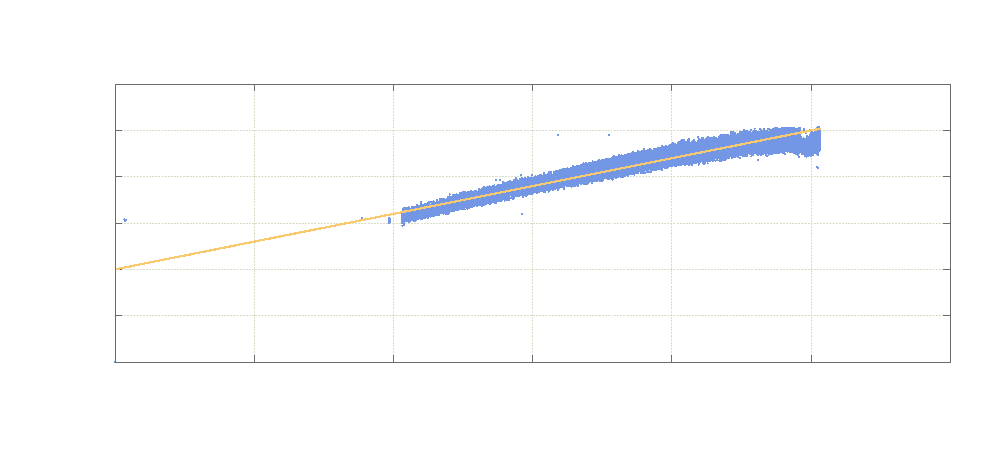
\includegraphics{Graphs/1/GuideVainPosition/GuideVainPosition}}%
    \gplfronttext
  \end{picture}%
\endgroup
}
			\caption{Modelling the compressor control from a guide vane\protect \footnotemark[1]}
			\label{fig: Guide vane position}
		\end{figure}
	
	\footnotetext[1]{Data recorded from a guide vane controlled compressor on a mine over a period of six months}
	
		In \gls{ptb}, the guide vane controller is modelled using a \gls{pi} controller. The non-linear limitations of guide vane control must be implemented in the controller. The control limitation is applied in the model by using a minimum control output limit that matches the minimum power reduction achieved by closing the guide vane to its minimum position. 
		\par 
		Mines utilise control valves at underground sections to adjust the pressure at individual mining stations independently \cite{Heyns2014Masters}. Controlling of valve components is performed similarly as control of the compressor components. \Cref{fig: Controller models} shows the outlet pressure is used as feedback for a \gls{pi} controller. The control output is mapped to the valve fraction of a pipe component.

		\begin{figure}[h]
			\centering
			\fbox{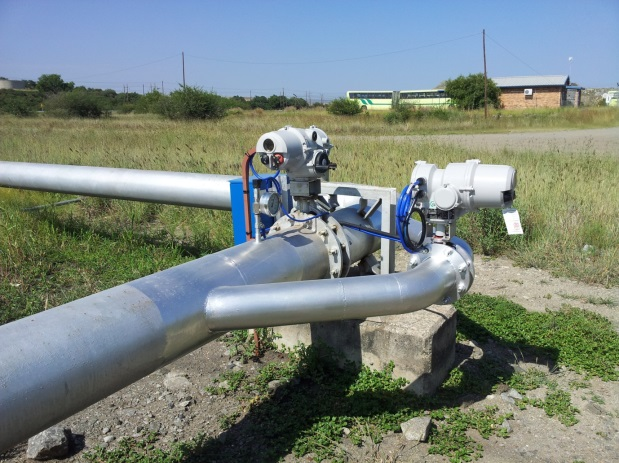
\includegraphics[ width=0.8\textwidth]{Images/3/Valve.jpg}}
			\caption[An example of a compressed air control valve]{An example of a compressed air control valve\cite{van2015implementation}} 
			\label{fig: Control}
		\end{figure}
		\subsubsection{Compressed air after-cooling}
		The air compression process generates significant heat. Compressed air at high temperatures contains a significant amount of water vapour. After-coolers are installed on compressed air systems to prevent condensation in the air network, improve the system capacity and to protect equipment from excessive heat \cite{schroeder2009energy}.
		\par 
		After-cooling reduces the compressed air temperature out of the compressors. This cooling can affect the operation of the network. Hence, including after-cooling to the simulation model should improve accuracy.
		\par
		Modelling the after-cooling is achieved in \gls{ptb} using a heat transfer node at the outlet of the compressor component model. The heat transfer parameters shown in \Cref{table: After cooling inputs} should be calibrated such that the air temperature matches after-cooled air temperature measurements. An assumption of 40 $^\circ$\gls{c} can be used if no measurements are available.
		\begin{table}
			\centering
			\begin{tabular}{lll}
				\hline 
				Parameter \hspace{1cm} & Definition \hspace{4cm} & Unit \\
				\hline
				$A$ & The heat transfer area & $m^2$ \\
				$UA$ & Heat transfer coefficient & $kW/^{\circ} C$ \\
				$T_{amb}$ & Ambient air temperature & $^{\circ} C$ \\
				\hline
			\end{tabular}
		\caption{The input parameters for the after-cooling simulation model}
		\label{table: After cooling inputs}
		\end{table}
	Depending on the accuracy requirement, after-cooling can be excluded from the simulation. Post after-cooling, compressed air is usually still warmer than ambient conditions. Air temperatures underground can be accurately matched by including heat transfer for compressed air pipelines.
	
	\subsection{Verify the simulation model}
	From the review of literature in \Cref{VerificationLit}, it was determined that \gls{mae} and the coefficient of determination are the most effective methods of measuring model accuracy. Therefore, for this study, both measures are utilised in the model verification. These measures are obtained by comparing the major simulation outputs (Total system power, flow and pressure) to actual data from the system. R-squared and \gls{mae} metrics are calculated by applying the applicable methodologies discussed in \Cref{VerificationLit}.	
	\par 
	For this study, the selected verification constraints were selected as : \\ {$r^2 > 0.9 $ and $ Err_{\%} < 5\% $}\\ If these limits are met for the power, flow and pressure of the system, the model is considered accurate. As an extra measure relative error of the output for the minor model components should be $ > 85\%$ of the actual data. To obtain the true error of the model, instrumentation measurement error should combined with the calculated simulation error.
	\par 
	Additionally, periodically repeated simulations could be used to verify simulations more definitively. To perform the repeated simulation verification, the input variables should be updated for each new period. The output values of the simulation should then be compared with actual measurements. For each simulation, the verification constraints should be met.
		
	\subsection{Select simulation inputs}
		The inputs of a simulation are any parameters that do not remain static or follow the same profile in day to day operation of the system. Examples of such parameters in a compressed air simulation are:
		\begin{itemize}
			\item Surface ambient conditions
			\item Machine operation schedules
			\item Air demands
			\item Operational changes
		\end{itemize} 
	Changing the simulation baseline period for a calibrated simulation should only require the updating of the input parameters. \Cref{fig: Compressor schedule} shows an example of a changing compressor schedule where an input parameter would need to be updated in the simulation.	

		\begin{figure}[h]
			\centering
			\fbox{% GNUPLOT: LaTeX picture with Postscript
\begingroup
  \makeatletter
  \providecommand\color[2][]{%
    \GenericError{(gnuplot) \space\space\space\@spaces}{%
      Package color not loaded in conjunction with
      terminal option `colourtext'%
    }{See the gnuplot documentation for explanation.%
    }{Either use 'blacktext' in gnuplot or load the package
      color.sty in LaTeX.}%
    \renewcommand\color[2][]{}%
  }%
  \providecommand\includegraphics[2][]{%
    \GenericError{(gnuplot) \space\space\space\@spaces}{%
      Package graphicx or graphics not loaded%
    }{See the gnuplot documentation for explanation.%
    }{The gnuplot epslatex terminal needs graphicx.sty or graphics.sty.}%
    \renewcommand\includegraphics[2][]{}%
  }%
  \providecommand\rotatebox[2]{#2}%
  \@ifundefined{ifGPcolor}{%
    \newif\ifGPcolor
    \GPcolortrue
  }{}%
  \@ifundefined{ifGPblacktext}{%
    \newif\ifGPblacktext
    \GPblacktextfalse
  }{}%
  % define a \g@addto@macro without @ in the name:
  \let\gplgaddtomacro\g@addto@macro
  % define empty templates for all commands taking text:
  \gdef\gplbacktext{}%
  \gdef\gplfronttext{}%
  \makeatother
  \ifGPblacktext
    % no textcolor at all
    \def\colorrgb#1{}%
    \def\colorgray#1{}%
  \else
    % gray or color?
    \ifGPcolor
      \def\colorrgb#1{\color[rgb]{#1}}%
      \def\colorgray#1{\color[gray]{#1}}%
      \expandafter\def\csname LTw\endcsname{\color{white}}%
      \expandafter\def\csname LTb\endcsname{\color{black}}%
      \expandafter\def\csname LTa\endcsname{\color{black}}%
      \expandafter\def\csname LT0\endcsname{\color[rgb]{1,0,0}}%
      \expandafter\def\csname LT1\endcsname{\color[rgb]{0,1,0}}%
      \expandafter\def\csname LT2\endcsname{\color[rgb]{0,0,1}}%
      \expandafter\def\csname LT3\endcsname{\color[rgb]{1,0,1}}%
      \expandafter\def\csname LT4\endcsname{\color[rgb]{0,1,1}}%
      \expandafter\def\csname LT5\endcsname{\color[rgb]{1,1,0}}%
      \expandafter\def\csname LT6\endcsname{\color[rgb]{0,0,0}}%
      \expandafter\def\csname LT7\endcsname{\color[rgb]{1,0.3,0}}%
      \expandafter\def\csname LT8\endcsname{\color[rgb]{0.5,0.5,0.5}}%
    \else
      % gray
      \def\colorrgb#1{\color{black}}%
      \def\colorgray#1{\color[gray]{#1}}%
      \expandafter\def\csname LTw\endcsname{\color{white}}%
      \expandafter\def\csname LTb\endcsname{\color{black}}%
      \expandafter\def\csname LTa\endcsname{\color{black}}%
      \expandafter\def\csname LT0\endcsname{\color{black}}%
      \expandafter\def\csname LT1\endcsname{\color{black}}%
      \expandafter\def\csname LT2\endcsname{\color{black}}%
      \expandafter\def\csname LT3\endcsname{\color{black}}%
      \expandafter\def\csname LT4\endcsname{\color{black}}%
      \expandafter\def\csname LT5\endcsname{\color{black}}%
      \expandafter\def\csname LT6\endcsname{\color{black}}%
      \expandafter\def\csname LT7\endcsname{\color{black}}%
      \expandafter\def\csname LT8\endcsname{\color{black}}%
    \fi
  \fi
    \setlength{\unitlength}{0.0500bp}%
    \ifx\gptboxheight\undefined%
      \newlength{\gptboxheight}%
      \newlength{\gptboxwidth}%
      \newsavebox{\gptboxtext}%
    \fi%
    \setlength{\fboxrule}{0.5pt}%
    \setlength{\fboxsep}{1pt}%
\begin{picture}(9360.00,4032.00)%
    \gplgaddtomacro\gplbacktext{%
      \colorrgb{0.00,0.00,0.00}%
      \put(550,924){\makebox(0,0)[r]{\strut{}}}%
      \colorrgb{0.00,0.00,0.00}%
      \put(550,1258){\makebox(0,0)[r]{\strut{}$1$}}%
      \colorrgb{0.00,0.00,0.00}%
      \put(550,1593){\makebox(0,0)[r]{\strut{}$2$}}%
      \colorrgb{0.00,0.00,0.00}%
      \put(550,1927){\makebox(0,0)[r]{\strut{}$3$}}%
      \colorrgb{0.00,0.00,0.00}%
      \put(550,2262){\makebox(0,0)[r]{\strut{}$4$}}%
      \colorrgb{0.00,0.00,0.00}%
      \put(550,2596){\makebox(0,0)[r]{\strut{}$5$}}%
      \colorrgb{0.00,0.00,0.00}%
      \put(550,2931){\makebox(0,0)[r]{\strut{}$6$}}%
      \colorrgb{0.00,0.00,0.00}%
      \put(550,3265){\makebox(0,0)[r]{\strut{}$7$}}%
      \colorrgb{0.00,0.00,0.00}%
      \put(550,3600){\makebox(0,0)[r]{\strut{}$8$}}%
      \colorrgb{0.00,0.00,0.00}%
      \put(682,704){\makebox(0,0){\strut{}00:00}}%
      \colorrgb{0.00,0.00,0.00}%
      \put(2062,704){\makebox(0,0){\strut{}04:00}}%
      \colorrgb{0.00,0.00,0.00}%
      \put(3442,704){\makebox(0,0){\strut{}08:00}}%
      \colorrgb{0.00,0.00,0.00}%
      \put(4822,704){\makebox(0,0){\strut{}12:00}}%
      \colorrgb{0.00,0.00,0.00}%
      \put(6202,704){\makebox(0,0){\strut{}16:00}}%
      \colorrgb{0.00,0.00,0.00}%
      \put(7582,704){\makebox(0,0){\strut{}20:00}}%
      \colorrgb{0.00,0.00,0.00}%
      \put(8962,704){\makebox(0,0){\strut{}00:00}}%
    }%
    \gplgaddtomacro\gplfronttext{%
      \csname LTb\endcsname%
      \put(176,2345){\rotatebox{-270}{\makebox(0,0){\strut{}Compressor}}}%
      \put(4822,374){\makebox(0,0){\strut{}Time of Day}}%
      \csname LTb\endcsname%
      \put(3967,100){\makebox(0,0)[r]{\strut{}Period 1}}%
      \csname LTb\endcsname%
      \put(5878,100){\makebox(0,0)[r]{\strut{}Period 2}}%
    }%
    \gplbacktext
    \put(0,0){
\includegraphics{Graphs/3/CompSelection/CompSelection}}%
    \gplfronttext
  \end{picture}%
\endgroup
}
			\caption{An example of two baseline periods, showing a changed compressor schedule}
			\label{fig: Compressor schedule}
		\end{figure}
	\subsection{Periodic simulation}	
		Periodic simulation refers to the repetition of simulations over subsequent periods to determine the sequential accuracy of the model. Sequential accuracy is important to verify the model is valid in general and not just a single period. This simulation will also indicate where operational changes have occurred as the simulation accuracy will be reduced.
		\par 
		The following process, as illustrated in \Cref{fig: PeriodicProcess}, was followed to implement periodic simulation: 
		\begin{itemize}
			\item Collect simulation input data periodically for each simulation interval
			\item Import input data series into simulation model
			\item Execute/solve the simulation
			\item Export the output simulation values
			\item Compare output data with the systems actual operation and identify major discrepancies
			\item Trigger the process periodically
		\end{itemize}
	%%%%%%%%%%%%%
	\clearpage
		\begin{figure}[h]
			\centering
			\fbox{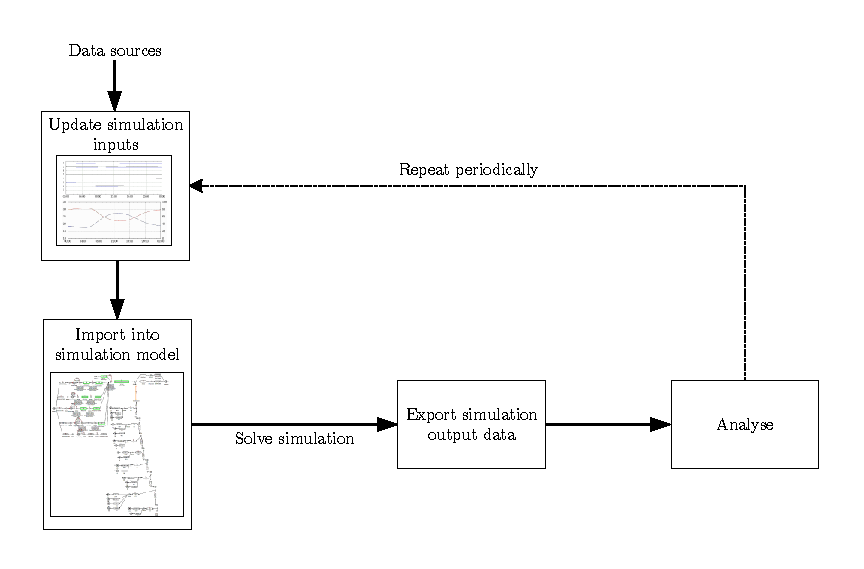
\includegraphics[trim =1.0cm 3.9cm 0.76cm 1cm,width=0.98\textwidth]{Graphs/4/PeriodicProcess/PeriodicProcess.pdf}}
			\caption{The periodic simulation process that was followed in this analysis}
			\label{fig: PeriodicProcess}
		\end{figure}
	
	
	\subsection{Summary}	
In this section, the subprocesses required for the simulation model development and verification were discussed. First, a method for selection of the model boundaries and parameters were discussed. A discussion on modelling procedure for compressed air sub-components then followed. The verification process and the selection of accuracy limits were then discussed concerning the analysis performed in section \Cref{VerificationLit}. The simulation input selection procedure was then reviewed. Finally, a procedure for repeated/periodic simulation was provided.

\section{Implement the simulation}
	\subsection{Preamble}
		Once a simulation has been developed and verified, the implementation of interventions and scenarios then follows. In this section, the approach of implementing the simulation methodology, and analysis of interventions will be discussed.
	\subsection{Execute simulation scenarios}
		At this point, the simulation model has been verified using historical data. The verified output data series is now used as a baseline upon which interventions can be quantified.  The simulation inputs of the model are now adjusted to create the desired scenario. For example to create a scenario where a specific compressor is shut down over a period, the input schedule of the compressor is adjusted in the simulation model.
		\par
		The simulation is then executed, and this process is repeated for each of the scenarios. For each scenario, the desired output parameters must be exported for further analysis.

	\subsection{Quantify operational benefit}
		With the data for each of the simulated scenarios exported, the relative improvement compared with the baseline should now be quantified. This comparison is achieved by analysing the differences between the baseline and optimised data series as shown visually in \Cref{fig: Savings Power.}.
		\begin{figure}[h]
			\centering
			% GNUPLOT: LaTeX picture with Postscript
\begingroup
  \makeatletter
  \providecommand\color[2][]{%
    \GenericError{(gnuplot) \space\space\space\@spaces}{%
      Package color not loaded in conjunction with
      terminal option `colourtext'%
    }{See the gnuplot documentation for explanation.%
    }{Either use 'blacktext' in gnuplot or load the package
      color.sty in LaTeX.}%
    \renewcommand\color[2][]{}%
  }%
  \providecommand\includegraphics[2][]{%
    \GenericError{(gnuplot) \space\space\space\@spaces}{%
      Package graphicx or graphics not loaded%
    }{See the gnuplot documentation for explanation.%
    }{The gnuplot epslatex terminal needs graphicx.sty or graphics.sty.}%
    \renewcommand\includegraphics[2][]{}%
  }%
  \providecommand\rotatebox[2]{#2}%
  \@ifundefined{ifGPcolor}{%
    \newif\ifGPcolor
    \GPcolortrue
  }{}%
  \@ifundefined{ifGPblacktext}{%
    \newif\ifGPblacktext
    \GPblacktextfalse
  }{}%
  % define a \g@addto@macro without @ in the name:
  \let\gplgaddtomacro\g@addto@macro
  % define empty templates for all commands taking text:
  \gdef\gplbacktext{}%
  \gdef\gplfronttext{}%
  \makeatother
  \ifGPblacktext
    % no textcolor at all
    \def\colorrgb#1{}%
    \def\colorgray#1{}%
  \else
    % gray or color?
    \ifGPcolor
      \def\colorrgb#1{\color[rgb]{#1}}%
      \def\colorgray#1{\color[gray]{#1}}%
      \expandafter\def\csname LTw\endcsname{\color{white}}%
      \expandafter\def\csname LTb\endcsname{\color{black}}%
      \expandafter\def\csname LTa\endcsname{\color{black}}%
      \expandafter\def\csname LT0\endcsname{\color[rgb]{1,0,0}}%
      \expandafter\def\csname LT1\endcsname{\color[rgb]{0,1,0}}%
      \expandafter\def\csname LT2\endcsname{\color[rgb]{0,0,1}}%
      \expandafter\def\csname LT3\endcsname{\color[rgb]{1,0,1}}%
      \expandafter\def\csname LT4\endcsname{\color[rgb]{0,1,1}}%
      \expandafter\def\csname LT5\endcsname{\color[rgb]{1,1,0}}%
      \expandafter\def\csname LT6\endcsname{\color[rgb]{0,0,0}}%
      \expandafter\def\csname LT7\endcsname{\color[rgb]{1,0.3,0}}%
      \expandafter\def\csname LT8\endcsname{\color[rgb]{0.5,0.5,0.5}}%
    \else
      % gray
      \def\colorrgb#1{\color{black}}%
      \def\colorgray#1{\color[gray]{#1}}%
      \expandafter\def\csname LTw\endcsname{\color{white}}%
      \expandafter\def\csname LTb\endcsname{\color{black}}%
      \expandafter\def\csname LTa\endcsname{\color{black}}%
      \expandafter\def\csname LT0\endcsname{\color{black}}%
      \expandafter\def\csname LT1\endcsname{\color{black}}%
      \expandafter\def\csname LT2\endcsname{\color{black}}%
      \expandafter\def\csname LT3\endcsname{\color{black}}%
      \expandafter\def\csname LT4\endcsname{\color{black}}%
      \expandafter\def\csname LT5\endcsname{\color{black}}%
      \expandafter\def\csname LT6\endcsname{\color{black}}%
      \expandafter\def\csname LT7\endcsname{\color{black}}%
      \expandafter\def\csname LT8\endcsname{\color{black}}%
    \fi
  \fi
    \setlength{\unitlength}{0.0500bp}%
    \ifx\gptboxheight\undefined%
      \newlength{\gptboxheight}%
      \newlength{\gptboxwidth}%
      \newsavebox{\gptboxtext}%
    \fi%
    \setlength{\fboxrule}{0.5pt}%
    \setlength{\fboxsep}{1pt}%
\begin{picture}(9360.00,3780.00)%
    \gplgaddtomacro\gplbacktext{%
      \colorrgb{0.00,0.00,0.00}%
      \put(682,924){\makebox(0,0)[r]{\strut{}$0$}}%
      \colorrgb{0.00,0.00,0.00}%
      \put(682,1788){\makebox(0,0)[r]{\strut{}$4$}}%
      \colorrgb{0.00,0.00,0.00}%
      \put(682,2651){\makebox(0,0)[r]{\strut{}$8$}}%
      \colorrgb{0.00,0.00,0.00}%
      \put(682,3515){\makebox(0,0)[r]{\strut{}$12$}}%
      \colorrgb{0.00,0.00,0.00}%
      \put(814,704){\makebox(0,0){\strut{}00:00}}%
      \colorrgb{0.00,0.00,0.00}%
      \put(2003,704){\makebox(0,0){\strut{}04:00}}%
      \colorrgb{0.00,0.00,0.00}%
      \put(3193,704){\makebox(0,0){\strut{}08:00}}%
      \colorrgb{0.00,0.00,0.00}%
      \put(4382,704){\makebox(0,0){\strut{}12:00}}%
      \colorrgb{0.00,0.00,0.00}%
      \put(5571,704){\makebox(0,0){\strut{}16:00}}%
      \colorrgb{0.00,0.00,0.00}%
      \put(6761,704){\makebox(0,0){\strut{}20:00}}%
      \colorrgb{0.00,0.00,0.00}%
      \put(7950,704){\makebox(0,0){\strut{}00:00}}%
      \colorrgb{0.00,0.00,0.00}%
      \put(8082,924){\makebox(0,0)[l]{\strut{}$0$}}%
      \colorrgb{0.00,0.00,0.00}%
      \put(8082,1572){\makebox(0,0)[l]{\strut{}$0.25$}}%
      \colorrgb{0.00,0.00,0.00}%
      \put(8082,2220){\makebox(0,0)[l]{\strut{}$0.5$}}%
      \colorrgb{0.00,0.00,0.00}%
      \put(8082,2867){\makebox(0,0)[l]{\strut{}$0.75$}}%
      \colorrgb{0.00,0.00,0.00}%
      \put(8082,3515){\makebox(0,0)[l]{\strut{}$1$}}%
    }%
    \gplgaddtomacro\gplfronttext{%
      \csname LTb\endcsname%
      \put(176,2219){\rotatebox{-270}{\makebox(0,0){\strut{}Power $(MW)$}}}%
      \put(8851,2219){\rotatebox{-270}{\makebox(0,0){\strut{}Power Saving $(MW)$}}}%
      \put(4382,374){\makebox(0,0){\strut{}Time of day}}%
      \csname LTb\endcsname%
      \put(2307,173){\makebox(0,0)[r]{\strut{}Baseline}}%
      \csname LTb\endcsname%
      \put(4746,173){\makebox(0,0)[r]{\strut{}Scenario}}%
      \csname LTb\endcsname%
      \put(7185,173){\makebox(0,0)[r]{\strut{}Power saving}}%
    }%
    \gplbacktext
    \put(0,0){\fbox{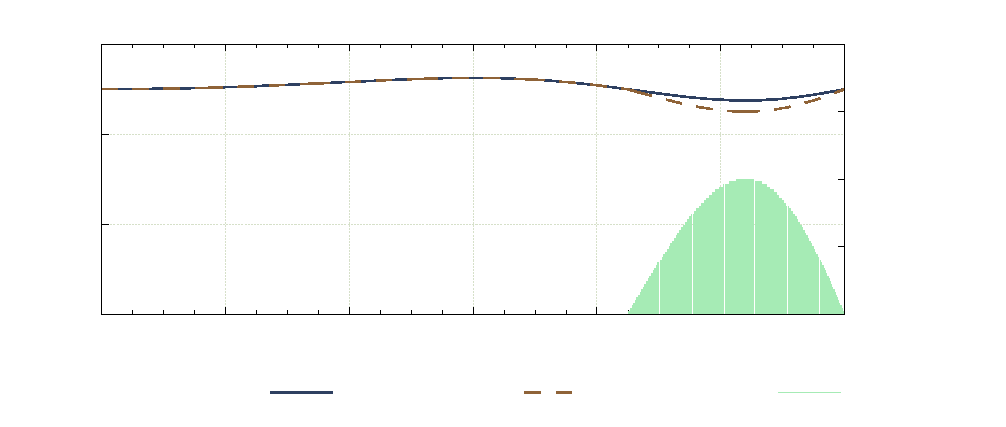
\includegraphics[trim=0 0 0.1cm 0, clip]{Graphs/3/savings/savings}}}%
    \gplfronttext
  \end{picture}%
\endgroup

			\caption{An example of a baseline vs. optimised power comparison}
			\label{fig: Savings Power.}
		\end{figure} 
		\footnotetext[1]{Eskom, "2017/18 Tariffs and charges" [Online] \url{http://www.eskom.co.za/CustomerCare/TariffsAndCharges/Pages/Tariffs_And_Charges.aspx}, [Accessed 28 June 2017]}
		
		For power data, the expected annual energy cost saving can be calculated using average weekday energy saving and the tariff structure provided by Eskom. The energy supplier's weekday \gls{tou} tariffs for both the high demand (Jun -- Aug) and low demand (Sep -- May) seasons are shown in \Cref{fig: Tariff}.
		\par 
		\begin{figure}[h]
			\centering
			% GNUPLOT: LaTeX picture with Postscript
\begingroup
  \makeatletter
  \providecommand\color[2][]{%
    \GenericError{(gnuplot) \space\space\space\@spaces}{%
      Package color not loaded in conjunction with
      terminal option `colourtext'%
    }{See the gnuplot documentation for explanation.%
    }{Either use 'blacktext' in gnuplot or load the package
      color.sty in LaTeX.}%
    \renewcommand\color[2][]{}%
  }%
  \providecommand\includegraphics[2][]{%
    \GenericError{(gnuplot) \space\space\space\@spaces}{%
      Package graphicx or graphics not loaded%
    }{See the gnuplot documentation for explanation.%
    }{The gnuplot epslatex terminal needs graphicx.sty or graphics.sty.}%
    \renewcommand\includegraphics[2][]{}%
  }%
  \providecommand\rotatebox[2]{#2}%
  \@ifundefined{ifGPcolor}{%
    \newif\ifGPcolor
    \GPcolortrue
  }{}%
  \@ifundefined{ifGPblacktext}{%
    \newif\ifGPblacktext
    \GPblacktextfalse
  }{}%
  % define a \g@addto@macro without @ in the name:
  \let\gplgaddtomacro\g@addto@macro
  % define empty templates for all commands taking text:
  \gdef\gplbacktext{}%
  \gdef\gplfronttext{}%
  \makeatother
  \ifGPblacktext
    % no textcolor at all
    \def\colorrgb#1{}%
    \def\colorgray#1{}%
  \else
    % gray or color?
    \ifGPcolor
      \def\colorrgb#1{\color[rgb]{#1}}%
      \def\colorgray#1{\color[gray]{#1}}%
      \expandafter\def\csname LTw\endcsname{\color{white}}%
      \expandafter\def\csname LTb\endcsname{\color{black}}%
      \expandafter\def\csname LTa\endcsname{\color{black}}%
      \expandafter\def\csname LT0\endcsname{\color[rgb]{1,0,0}}%
      \expandafter\def\csname LT1\endcsname{\color[rgb]{0,1,0}}%
      \expandafter\def\csname LT2\endcsname{\color[rgb]{0,0,1}}%
      \expandafter\def\csname LT3\endcsname{\color[rgb]{1,0,1}}%
      \expandafter\def\csname LT4\endcsname{\color[rgb]{0,1,1}}%
      \expandafter\def\csname LT5\endcsname{\color[rgb]{1,1,0}}%
      \expandafter\def\csname LT6\endcsname{\color[rgb]{0,0,0}}%
      \expandafter\def\csname LT7\endcsname{\color[rgb]{1,0.3,0}}%
      \expandafter\def\csname LT8\endcsname{\color[rgb]{0.5,0.5,0.5}}%
    \else
      % gray
      \def\colorrgb#1{\color{black}}%
      \def\colorgray#1{\color[gray]{#1}}%
      \expandafter\def\csname LTw\endcsname{\color{white}}%
      \expandafter\def\csname LTb\endcsname{\color{black}}%
      \expandafter\def\csname LTa\endcsname{\color{black}}%
      \expandafter\def\csname LT0\endcsname{\color{black}}%
      \expandafter\def\csname LT1\endcsname{\color{black}}%
      \expandafter\def\csname LT2\endcsname{\color{black}}%
      \expandafter\def\csname LT3\endcsname{\color{black}}%
      \expandafter\def\csname LT4\endcsname{\color{black}}%
      \expandafter\def\csname LT5\endcsname{\color{black}}%
      \expandafter\def\csname LT6\endcsname{\color{black}}%
      \expandafter\def\csname LT7\endcsname{\color{black}}%
      \expandafter\def\csname LT8\endcsname{\color{black}}%
    \fi
  \fi
    \setlength{\unitlength}{0.0500bp}%
    \ifx\gptboxheight\undefined%
      \newlength{\gptboxheight}%
      \newlength{\gptboxwidth}%
      \newsavebox{\gptboxtext}%
    \fi%
    \setlength{\fboxrule}{0.5pt}%
    \setlength{\fboxsep}{1pt}%
\begin{picture}(9360.00,4032.00)%
    \gplgaddtomacro\gplbacktext{%
      \colorrgb{0.00,0.00,0.00}%
      \put(814,924){\makebox(0,0)[r]{\strut{}$0$}}%
      \colorrgb{0.00,0.00,0.00}%
      \put(814,1398){\makebox(0,0)[r]{\strut{}$50$}}%
      \colorrgb{0.00,0.00,0.00}%
      \put(814,1872){\makebox(0,0)[r]{\strut{}$100$}}%
      \colorrgb{0.00,0.00,0.00}%
      \put(814,2345){\makebox(0,0)[r]{\strut{}$150$}}%
      \colorrgb{0.00,0.00,0.00}%
      \put(814,2819){\makebox(0,0)[r]{\strut{}$200$}}%
      \colorrgb{0.00,0.00,0.00}%
      \put(814,3293){\makebox(0,0)[r]{\strut{}$250$}}%
      \colorrgb{0.00,0.00,0.00}%
      \put(814,3767){\makebox(0,0)[r]{\strut{}$300$}}%
      \colorrgb{0.00,0.00,0.00}%
      \put(946,704){\makebox(0,0){\strut{}00:00}}%
      \colorrgb{0.00,0.00,0.00}%
      \put(2282,704){\makebox(0,0){\strut{}04:00}}%
      \colorrgb{0.00,0.00,0.00}%
      \put(3618,704){\makebox(0,0){\strut{}08:00}}%
      \colorrgb{0.00,0.00,0.00}%
      \put(4954,704){\makebox(0,0){\strut{}12:00}}%
      \colorrgb{0.00,0.00,0.00}%
      \put(6290,704){\makebox(0,0){\strut{}16:00}}%
      \colorrgb{0.00,0.00,0.00}%
      \put(7626,704){\makebox(0,0){\strut{}20:00}}%
      \colorrgb{0.00,0.00,0.00}%
      \put(8962,704){\makebox(0,0){\strut{}00:00}}%
    }%
    \gplgaddtomacro\gplfronttext{%
      \csname LTb\endcsname%
      \put(176,2345){\rotatebox{-270}{\makebox(0,0){\strut{}c/kWhr}}}%
      \put(4954,374){\makebox(0,0){\strut{}Time of Day}}%
      \csname LTb\endcsname%
      \put(4219,173){\makebox(0,0)[r]{\strut{}High demand season}}%
      \csname LTb\endcsname%
      \put(7132,173){\makebox(0,0)[r]{\strut{}Low demand season}}%
    }%
    \gplbacktext
        \put(0,0){\fbox{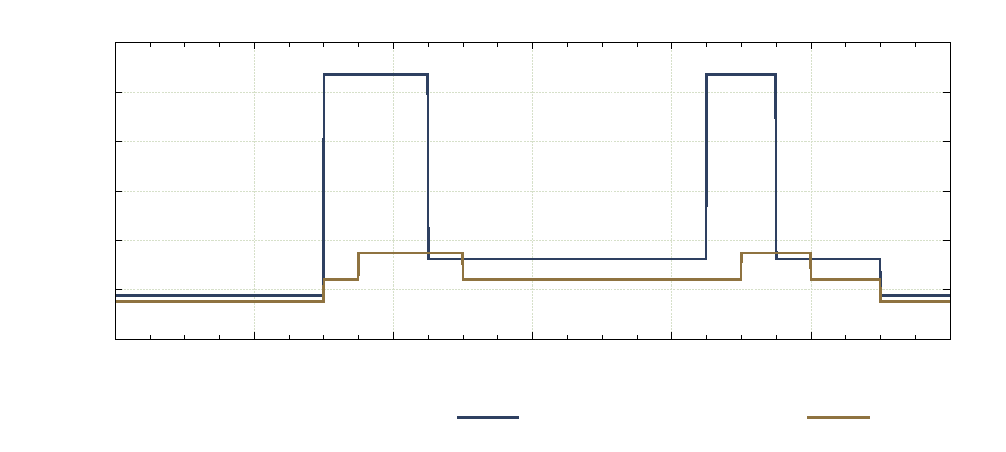
\includegraphics[trim=0 0 0.1cm 0, clip]{Graphs/3/tariff/tariff}}}%
    \gplfronttext
  \end{picture}%
\endgroup

			\caption[Eskom's weekday TOU tariff structure]{Eskom's weekday \gls{tou} tariff structure.\protect \footnotemark[1]}
			\label{fig: Tariff}
		\end{figure}
		
		Estimating the cost-benefit for improvements in pressure delivery is harder to quantify. Instead, the average pressure benefit for a period should be provided in kPa. For example, \enquote{The simulation indicated an $x$ MW saving with an additional pressure improvement of $y$ kPa during the drilling shift}.

		\subsection{Report results to the mine}
		Once the benefits for each simulated scenario has been calculated and quantified, the interventions should be prioritised in the order of the greatest benefit for the mine. The implementation costs and pay back periods of the interventions can also be considered in this process.
		\par
		The results and recommendations should be submitted to responsible mine personnel in the form of a report; an example report is shown in \Cref{fig: Report example}. At this point, the process of implementation becomes the mine's responsibility. The mine may require further validation of the results through practical testing.
		\begin{figure}[h]
			\centering
			\fbox{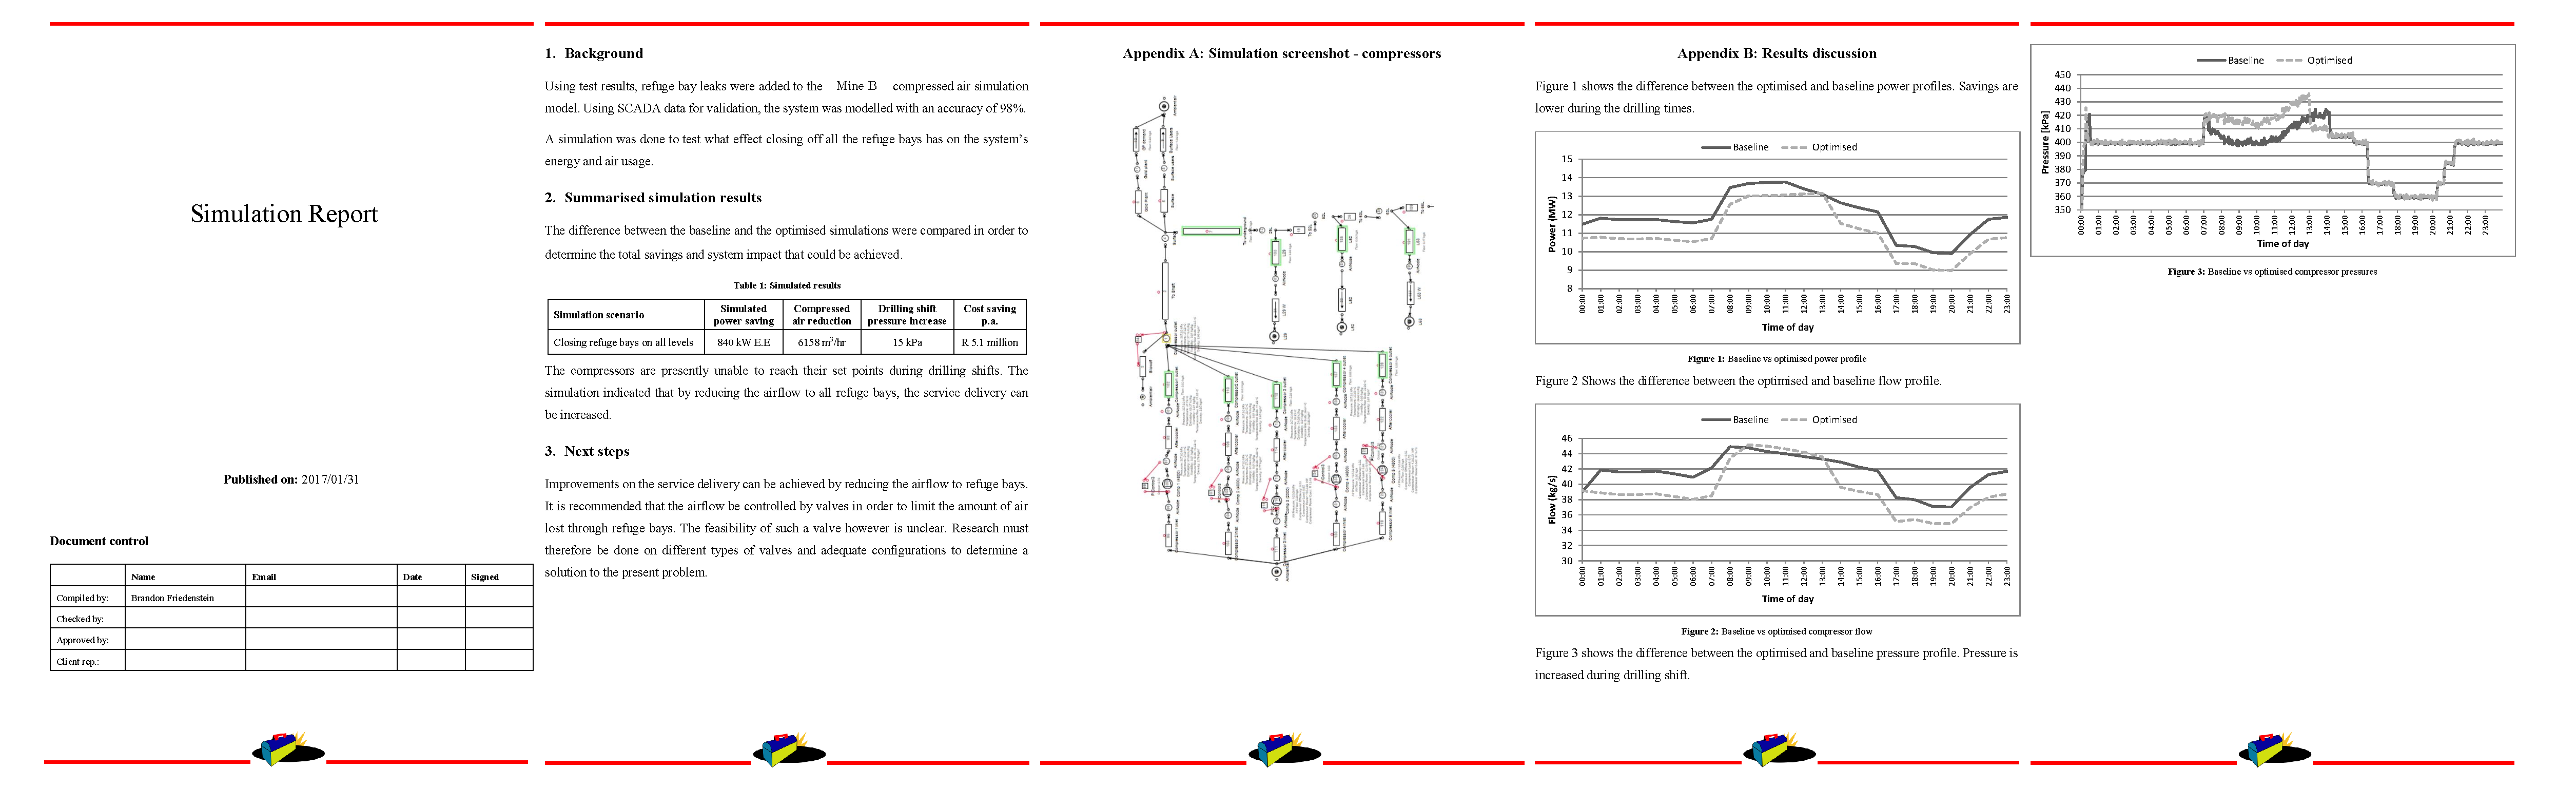
\includegraphics[width=0.98\textwidth]{Images/3/ReportExample.pdf}}
			\caption{An example of a simulation report that is submitted to the mine personnel}
			\label{fig: Report example}
		\end{figure}

	\subsection{Summary}
	This section discussed the of implantation of the simulation procedure. Implementation involves execution of the simulation scenarios, followed by the numerical calculation and quantification of energy cost savings and other benefits. Finally, the procedure to report findings to the mine is given.
\section{Conclusion}
The aim of chapter 3 was to provide a methodology to develop compressed air simulations. The method was  broken into three steps:
\begin{enumerate}
	\item Investigate the system
	\item Develop and verify a simulation model
	\item Execute the simulated scenarios and quantify the benefits
\end{enumerate}
This investigation step involved obtaining and verifying data and information regarding the compressed air network. Processes to resolve scenarios where data can not be obtained were also provided.
\par 
In the next step, a simulation model development and verification procedure were provided. This procedure also described the selection of model and simulation parameters, the development of subcomponent models as well as a verification procedure A methodology for repeated/periodic simulation was also provided.
\par 
The final step involved the execution of the simulation followed by the methods to calculate, quantify and report potential benefits of the simulated scenarios.
